%% RSAA THESIS 'TEMPLATE' BY JOSHUA RICH <joshua.rich@gmail.com>
%% README:
% This template is designed to be used with pdflatex rather than plain
% latex.  It was developed under a TeXLive 2007 TeX distribution on
% Linux.  

% for requirements of typesetting and formatting see:
% http://info.anu.edu.au/Policies/_REG/Guidelines/PhD_Exam_Theses.asp
% (in emacs, type M-x browse-url with the cursor on 
% the link above)

%%NOTES ABOUT THE DOCUMENT CLASS
% Yes, I'm using a report style.  Any 'thesis style' you might
% find or someone will give you is based on the standard report
% class, but is probably well outdated compared to whatever TeX
% you have installed.  Besides, why use that style file if you 
% have no idea what it actually does?  You will probably just redefine
% all of its customisations anyway...
\documentclass[12pt,openright]{report} 

% define some constants that can be used in various places to easily
% specify title, subjects, author etc.
\newcommand{\thesistitle}{Type Ia Supernova Physics}
\newcommand{\fullname}{Wolfgang Eitel Kerzendorf}
\newcommand{\shortname}{W. E. Kerzendorf}
\newcommand{\thesissubjects}{supernova:progenitors ????add some more?????}

%%NOTES ABOUT BABEL PACKAGE:
% It requires two components; the 
% \usepackage line above and the language put in the \documentclass.
% 'british' is used because that is the english style required for an
% ANU thesis.  This will ensure LaTeX uses british hyphenation and
% other language constructs when generating the text.  Putting the
% babel usepackage at the very top also ensures other packages called
% through \usepackage can take advantage of babel if they are set up
% for such.  
% We can also do tricky things in our ~/.emacs file if we
% are an emacs user now as well.  Grab the flyspell-babel and
% ispell-multi  emacs packages from:
% http://www.dur.ac.uk/p.j.heslin/Software/Emacs/
% And put it somewhere Emacs can find it (probably under ~/.emacs.d).
% Then add the following lines to your .emacs:
%   (dolist (hook '(LaTeX-mode-hook))
%   (add-hook hook (lambda () (flyspell-mode 1))))
%   (add-hook 'tex-mode-hook (function (lambda () (setq ispell-parser 'tex))))
%   (autoload 'flyspell-babel-setup "flyspell-babel")
%   (add-hook 'latex-mode-hook 'flyspell-babel-setup)
% After this, you should have Emacs auto-suggesting word corrections
% AND doing it in british-english automagically.  You can do a similar trick
% for papers by simply changing 'british' above to 'american', and
% flyspell will check your paper in american-english.
\usepackage[british]{babel}


% ---------------------------------------------------------------------
% page size and margins
% ---------------------------------------------------------------------
%%NOTES ABOUT GEOMETRY PACKAGE:
% Below is using the geometry package as it is just cool.  This allows
% you to directly specify the margin requirements as outlined by ANU
% directly.  Here the inner border is 4cm and the outer is 2cm.  Top
% and bottom are also 2cm.  This is much easier than trying to work
% out page and margin dimensions by hand.  This is how you should use
% LaTeX...
\usepackage{geometry}
\geometry{a4paper,twoside}
\geometry{includehead,includefoot}
\geometry{hmargin={4cm,2cm}}
\geometry{vmargin={2cm,2cm}}

% ---------------------------------------------------------------------
% miscellaneous packages used
% ---------------------------------------------------------------------
\usepackage[hiresbb]{graphicx}
\DeclareGraphicsExtensions{.pdf}
%\DeclareGraphicsExtensions{.eps}
\usepackage[twoside]{rotating}
%%NOTES ABOUT FONTS PACKAGES:
% The basic requirements for fonts in an ANU thesis demand clear
% readability and that is about all.  So if you choose a nice,
% standard serif font you won't have any problems.
% I several font families in my thesis below:
%  pxfonts: math typesetting
%  tgpagella: for the normal text font (serif)
%  tgheros: for the sans serif font
%  tgcursor: for the typewriter style font
% TeX Gyre Pagella, Heros and Cursor are part of the TeX Gyre family
% of fonts, which can be obtained from:
%   http://www.gust.org.pl/projects/e-foundry/tex-gyre/
% Not all of the TeX Gyre, and possibly not the latest glyphs are
% available in standard TeX distributions.  
%
% The 'mathpazo' package provides an almost identical, albeit not
% actively developed font family to TeX Gyre Pagella and is included
% in standard TeX distributions.  This package
% also provides a full range of math glyphs.  You'd need to find
% alternative sans serif and typewriter fonts to use with this package.
%
% You can see a whole heap of LaTeX fonts, most of which are also in a
% standard TeX distribution at: 
%  http://www.tug.dk/FontCatalogue/
% This web-page shows what each font looks like and what you need to
% do to include the font in your document.  Note it lists fonts that
% may not be installed by your default TeX installation...
%
% Another list of fonts, recommended by `typophiles' can be found at:
%  http://typophile.com/node/18207
% Although the above list includes some really nice fonts, their
% availability in TeX distributions varies.  You may have to install
% them manually...
\usepackage[T1]{fontenc}
\usepackage{textcomp}
\usepackage{ucs}
\usepackage[utf8x]{inputenc}
\usepackage{amsmath,amssymb}
\usepackage{pxfonts}
\usepackage{tgheros,tgpagella}
\renewcommand*\ttdefault{qcr}
\linespread{1.05} % tgpagella/mathpazo need a bigger line spacing
\usepackage{microtype}
% bibliography uses natbib, this will be a requirement
\usepackage[round]{natbib}
% Super-nice looking tables, better than deluxetable
\usepackage{longtable,booktabs,multirow}
%%NOTES ABOUT CAPTION AND SUBFIG PACKAGES
% I'm using the caption package to style my captions.
% You need to read the documentation for this package (on CTAN) as it
% has simple explanations of the options and examples of what it looks
% like.
%
% The subfig package allows the ability to control in detail
% positioning of sub-plots in a complex figure as well as add labels
% to them, which can then be referenced in the text without the need
% for changing the actual number as your sub-figures change.
% The subfig package inherits options from the caption package, so
% declare them together.
%
\usepackage[]{caption,subfig}
\captionsetup{format=hang,%
  indention=-1.5cm,%
  labelsep=quad,%
  labelfont={footnotesize,bf},%
  textfont={footnotesize}}
% The hyperref package is a must while editing.  It provides urls
% inside your document; you can then click to go to certain pages,
% figures or bibliography entries.
\usepackage[unicode,pageanchor,colorlinks,plainpages=false]{hyperref}
% \hypersetup{pdftitle=\thesistitle\ - \shortname,%
%   pdfauthor=\fullname,%
%   pdfsubject={\thesissubjects},%
%   citecolor=DodgerBlue3,%
%   linkcolor=Ivory4,%
%   anchorcolor=CadetBlue4}
%for printing, make all colours black...
\hypersetup{pdftitle=\thesistitle\ - \shortname,%
  pdfauthor=\fullname,%
  pdfsubject={\thesissubjects},%
  citecolor=black,%
  filecolor=black,%
  linkcolor=black,%
  urlcolor=black%
}
% Drop capitals at the start of chapters
\usepackage{lettrine}
% Allow defining of colours. Useful for:
% - defining the colours of links, citations etc.
% together with hyperref (i.e. in hyperrefsetup)
% - get alternating row colours or shades in tables
\usepackage[hyperref,x11names]{xcolor}
% Stops figures and tables 'floating' past the section in which they
% are declared.
\usepackage[section]{placeins}
\usepackage[toc,page,title,titletoc]{appendix}
%%NOTES ABOUT NAG
% this is a very good package to use.  If you want to write good LaTeX
% code and want to make sure you aren't using outdated methods (like
% your supervisor does), then use this package.  It will complain when
% you use outdated or wrong LaTeX commands.
\usepackage[l2tabu, orthodox]{nag}
\usepackage{ifthen}

% ---------------------------------------------------------------------
% styles for header, footer, pages, bibliography
% ---------------------------------------------------------------------
%

% chapter heading style
% this is the 'Conny' style from the fncychap package, modified to
% remove the two bold lines before the 'Chapter X' title.
% For usage of this package, see:
%  http://tug.ctan.org/cgi-bin/ctanPackageInformation.py?id=fncychap
%
\usepackage{fncychap}
\makeatletter
\ChNameUpperCase
\ChTitleUpperCase  
\ChNameVar{\centering\Huge\usefont{OT1}{qbk}{m}{n}\selectfont}
\ChNumVar{\Huge}
\ChTitleVar{\centering\Huge\usefont{OT1}{qbk}{m}{n}\selectfont}
\ChRuleWidth{2pt}
\renewcommand{\DOCH}{%
  \CNV\FmN{\@chapapp}\space \CNoV\thechapter
  \par\nobreak
  \vskip -0.5\baselineskip
}
\renewcommand{\DOTI}[1]{%
  \mghrulefill{\RW}\par\nobreak
  \CTV\FmTi{#1}\par\nobreak
  \vskip 60\p@
}
\renewcommand{\DOTIS}[1]{%
  \mghrulefill{\RW}\par\nobreak
  \CTV\FmTi{#1}\par\nobreak
  \vskip 60\p@
}

%
%%% page styles:
%
\usepackage{fancyhdr}
\fancyhead{}
\fancyfoot{}
%% make the odd pages have the section name on the top right
%\fancyhead[RO]{\usefont{OT1}{qbk}{m}{n}\selectfont \rightmark}
%% make the even pages have the chapter name on the top left
%\fancyhead[LE]{\usefont{OT1}{qbk}{m}{n}\selectfont \leftmark}
%
% fancy (main content) page header/footer styles
\fancyfoot[LE]{\usefont{OT1}{qbk}{m}{n}\selectfont \thepage}
\fancyfoot[RO]{\usefont{OT1}{qbk}{m}{n}\selectfont \thepage}
\renewcommand{\footrulewidth}{0.5pt}
\renewcommand{\footruleskip}{0mm}
% plain page header/footer styles (i.e. chapter pages)
\fancypagestyle{plain}{
\fancyhf{}
\fancyfoot[LE]{\usefont{OT1}{qbk}{m}{n}\selectfont \thepage}
\fancyfoot[RO]{\usefont{OT1}{qbk}{m}{n}\selectfont \thepage}
\renewcommand{\headrulewidth}{0pt}
\renewcommand{\footrulewidth}{0pt}
}

%
% this next section (till \makeatother) makes sure that blank pages
% are actually completely blank, cause they're not usually
\makeatletter
\def\cleardoublepage{\clearpage\if@twoside \ifodd\c@page\else
	\hbox{}
	\vspace*{\fill}
	\thispagestyle{empty}
	\newpage
	\if@twocolumn\hbox{}\newpage\fi\fi\fi}
\makeatother

%
%%% section header styles:
%
\usepackage[calcwidth]{titlesec}
\titlelabel{\thetitle.\quad}


%\includeonly{macros,chapter1}
%\includeonly{macros,chapter2}
%\includeonly{macros,chapter3}
%\includeonly{macros,chapter4}

% uncomment if you would like an index (make sure you actually define
% index terms in your document as well...
%\makeindex

% this contains various command definitions and other misc. options
% ---------------------------------------------------------------------
% command re-definitions and additions
% ---------------------------------------------------------------------

% i.e. -- e.g. -- etc. -- et. al.
\newcommand{\eg}{{\em e.g.,}}
\newcommand{\ie}{{\em i.e.,}}
\newcommand{\etc}{{\em etc.}}
\newcommand{\etal}{{\em et al.}}

% symbols
\newcommand{\HI}{\hbox{\rmfamily H\,{\textsc i}}}
\newcommand{\HIfat}{\hbox{\rmfamily\bfseries H\,{\textsc i}}}
\newcommand{\HIsub}{\hbox{{\scriptsize H}\,{\tiny I}}}
\newcommand{\HII}{\hbox{\rmfamily H\,{\scshape ii}}}
\newcommand{\HIIsub}{\hbox{\scriptsize \rmfamily H\,{\scshape ii}}}
\newcommand{\Ha}{\hbox{\rmfamily H\,$\alpha$}}
\newcommand{\msun}{\hbox{$M_{\odot}$}}
\newcommand{\mhi}{\hbox{$M_{\HIsub}$}}
\newcommand{\lsun}{\hbox{$L_{\odot}$}}
\newcommand{\mlsun}{(M/L)_{\odot}}
\newcommand{\vexp}{\hbox{$V_{exp}$}}
\newcommand{\vhel}{\hbox{$V_{hel}$}}
\newcommand{\vdisp}{\hbox{$\sigma_{disp}$}}
\newcommand{\Nhi}{\hbox{$N_{\HIsub}$}}
\newcommand{\nhi}{\hbox{$n_{\HIsub}$}}
\newcommand{\Mhi}{\hbox{$M_{\HIsub}$}}
\newcommand{\ra}{$\alpha$}
\newcommand{\dec}{$\delta$}
\newcommand{\degree}{\textdegree}
\newcommand{\arcmin}{\hbox{$^\prime$}}
\newcommand{\arcsec}{\hbox{$^{\prime\prime}$}}
\newcommand{\kms}{\hbox{km s$^{-1}$}}
\newcommand{\mjbeam}{\hbox{mJy beam$^{-1}$}}
\newcommand{\jbeam}{\hbox{Jy beam$^{-1}$}}
\newcommand{\mjbeamkms}{\hbox{mJy/beam km s$^{-1}$}}
\newcommand{\jkms}{\hbox{Jy km s$^{-1}$}}
\newcommand{\coldensity}{\hbox{cm$^{-2}$}}
\newcommand{\voldensity}{\hbox{cm$^{-3}$}}
% add others you need

% footnote symbols
% use \symbolfootnote[1]{footnote} to get an *
%     * 1 - *
%     * 2 - dagger
%     * 3 - double dagger
%     * 4 - ... 9 (see page 175 of the latex manual) 
\long\def\symbolfootnote[#1]#2{\begingroup%
\def\thefootnote{\fnsymbol{footnote}}\footnote[#1]{#2}\endgroup}
% New definition of square root:
% it renames \sqrt as \oldsqrt
% it defines the new \sqrt in terms of the old one
% See:
%  http://en.wikibooks.org/wiki/LaTeX/Tips_and_Tricks#New_Square_Root
\let\oldsqrt\sqrt
\def\sqrt{\mathpalette\DHLhksqrt}
\def\DHLhksqrt#1#2{%
\setbox0=\hbox{$#1\oldsqrt{#2\,}$}\dimen0=\ht0
\advance\dimen0-0.2\ht0
\setbox2=\hbox{\vrule height\ht0 depth -\dimen0}%
{\box0\lower0.4pt\box2}}
% define a new url command so a nice font can be used
\newcommand{\myurl}[1]{\small\texttt{#1}}
% handy referencing of figures/tables, see 'Guide to using Encapsulated
% PostScript in LaTeX.', Section 17.1.1
\newcommand\FigDiff[1]{\hyperref[#1]{Figure~\ref*{#1}} on Page~\pageref*{#1}}
\newcommand\FigSame[1]{\hyperref[#1]{Figure~\ref*{#1}}}
\newcommand\Figref[1]{\ifthenelse{\value{page}=\pageref{#1}}
                     {\FigSame{#1}}{\FigDiff{#1}}}
\newcommand\TabDiff[1]{\hyperref[#1]{Table~\ref*{#1}} on Page~\pageref*{#1}}
\newcommand\TabSame[1]{\hyperref[#1]{Table~\ref*{#1}}}
\newcommand\Tabref[1]{\ifthenelse{\value{page}=\pageref{#1}}
                     {\TabSame{#1}}{\TabDiff{#1}}}

% text to add to end of continued figures caption
\newcommand\ContFig[1]{\textit{(Figure continued from page \pageref*{#1})}}

% ---------------------------------------------------------------------
% pdflatex setup
% ---------------------------------------------------------------------
% make pdflatex use the same spacing (paragraph, line and page breaks)
% as standard LaTeX 
\pdfadjustspacing=1

% ---------------------------------------------------------------------
%  misc. options
% ---------------------------------------------------------------------
% table of contents will go to subsubsections
\setcounter{tocdepth}{3}  

% ---------------------------------------------------------------------
% more liberal 'float' (tables, figures) placement
% ---------------------------------------------------------------------
% Alter some LaTeX defaults for better treatment of figures:
% See p.105 of "TeX Unbound" for suggested values.
% See pp. 199-200 of Lamport's "LaTeX" book for details.
% General parameters, for ALL pages:
\renewcommand{\topfraction}{0.9}	% max fraction of floats at top
\renewcommand{\bottomfraction}{0.8}	% max fraction of floats at bottom
% Parameters for TEXT pages (not float pages):
\setcounter{topnumber}{2}
\setcounter{bottomnumber}{2}
\setcounter{totalnumber}{4}     % 2 may work better
\setcounter{dbltopnumber}{2}    % for 2-column pages
\renewcommand{\dbltopfraction}{0.9}	% fit big float above 2-col. text
\renewcommand{\textfraction}{0.07}	% allow minimal text w. figs
% Parameters for FLOAT pages (not text pages):
\renewcommand{\floatpagefraction}{0.7}	% require fuller float pages
% N.B.: floatpagefraction MUST be less than topfraction !!
\renewcommand{\dblfloatpagefraction}{0.7}	% require fuller float pages
% remember to use [htp] or [htpb] for placement

% ---------------------------------------------------------------------
% Journal name abbreviations
% ---------------------------------------------------------------------
\newcommand{\jnlref}[1]{\textrm{#1}}
\newcommand{\aj}{\jnlref{AJ}}
\newcommand{\araa}{\jnlref{ARA\&A}}
\newcommand{\apj}{\jnlref{ApJ}}
\newcommand{\apjl}{\jnlref{ApJ}}
\newcommand{\apjs}{\jnlref{ApJS}}
\newcommand{\ao}{\jnlref{Appl.~Opt.}}
\newcommand{\apss}{\jnlref{Ap\&SS}}
\newcommand{\aap}{\jnlref{A\&A}}
\newcommand{\aapr}{\jnlref{A\&A~Rev.}}
\newcommand{\aaps}{\jnlref{A\&AS}}
\newcommand{\azh}{\jnlref{AZh}}
\newcommand{\baas}{\jnlref{BAAS}}
\newcommand{\jrasc}{\jnlref{JRASC}}
\newcommand{\memras}{\jnlref{MmRAS}}
\newcommand{\mnras}{\jnlref{MNRAS}}
\newcommand{\pra}{\jnlref{Phys.~Rev.~A}}
\newcommand{\prb}{\jnlref{Phys.~Rev.~B}}
\newcommand{\prc}{\jnlref{Phys.~Rev.~C}}
\newcommand{\prd}{\jnlref{Phys.~Rev.~D}}
\newcommand{\pre}{\jnlref{Phys.~Rev.~E}}
\newcommand{\prl}{\jnlref{Phys.~Rev.~Lett.}}
\newcommand{\pasp}{\jnlref{PASP}}
\newcommand{\pasj}{\jnlref{PASJ}}
\newcommand{\qjras}{\jnlref{QJRAS}}
\newcommand{\skytel}{\jnlref{S\&T}}
\newcommand{\solphys}{\jnlref{Sol.~Phys.}}
\newcommand{\sovast}{\jnlref{Soviet~Ast.}}
\newcommand{\ssr}{\jnlref{Space~Sci.~Rev.}}
\newcommand{\zap}{\jnlref{ZAp}}
\newcommand{\nat}{\jnlref{Nature}}
\newcommand{\iaucirc}{\jnlref{IAU~Circ.}}
\newcommand{\aplett}{\jnlref{Astrophys.~Lett.}}
\newcommand{\apspr}{\jnlref{Astrophys.~Space~Phys.~Res.}}
\newcommand{\bain}{\jnlref{Bull.~Astron.~Inst.~Netherlands}}
\newcommand{\fcp}{\jnlref{Fund.~Cosmic~Phys.}}
\newcommand{\gca}{\jnlref{Geochim.~Cosmochim.~Acta}}
\newcommand{\grl}{\jnlref{Geophys.~Res.~Lett.}}
\newcommand{\jcp}{\jnlref{J.~Chem.~Phys.}}
\newcommand{\jgr}{\jnlref{J.~Geophys.~Res.}}
\newcommand{\jqsrt}{\jnlref{J.~Quant.~Spec.~Radiat.~Transf.}}
\newcommand{\memsai}{\jnlref{Mem.~Soc.~Astron.~Italiana}}
\newcommand{\nphysa}{\jnlref{Nucl.~Phys.~A}}
\newcommand{\physrep}{\jnlref{Phys.~Rep.}}
\newcommand{\physscr}{\jnlref{Phys.~Scr}}
\newcommand{\planss}{\jnlref{Planet.~Space~Sci.}}
\newcommand{\procspie}{\jnlref{Proc.~SPIE}}
\newcommand{\ieeesigprocm}{\jnlref{IEEE~Signal~Processing~Magazine}}
\newcommand{\cjaa}{\jnlref{Chinese J. Astron. Astrophys.}}
\let\astap=\aap
\let\apjlett=\apjl
\let\apjsupp=\apjs
\let\applopt=\ao

%%% Local Variables:
%%% TeX-master: "thesis.tex"
%%% End:


\begin{document}

\pagestyle{empty}

%
%%% TITLE PAGE:
%
% This title-page is based on many bits of information found on the
% Internet by searching for 'thesis title page latex'.  Packages are
% also available on CTAN if you don't like this style and don't feel
% confident creating a style yourself.
%
% Remove or change the \usefont..\selectfont if you don't have the
% TeX Gyre Bonum font.
%
\begin{titlepage}\usefont{OT1}{qbk}{m}{n}\selectfont
  \begin{center}
    \LARGE{\thesistitle}
    \\[2cm]
    \Large{\fullname}
    \\[2cm]
    \normalsize{A thesis submitted for the degree of\\[0.5cm]
      Doctor of Philosophy\\[0.5cm]
      of The Australian National University}
    \\[1.5cm]
    
\includegraphics[width=0.5\textwidth]{anu-logo-colour}
    \\[1.5cm]
    \large{Research School of Astronomy and Astrophysics \\[0.25cm]
      The Australian National University \\[0.25cm]
      Canberra ACT 0200 \\[0.25cm]
      Australia}
    \\[2cm]
    \textsf{October 2008}
  \end{center}
\end{titlepage}

%
%%% DEDICATION:
%
% dedication page
\begin{figure}
\centering
{\large\usefont{OT1}{qzc}{m}{n}\selectfont
Fancy schmancy italic text for a dedication.}
\end{figure}


%
%%% FRONT CONTENT:
%
% page numbering as roman numerals
% don't indent paragraphs 
% increase the amount of space between paragraphs
\pagestyle{plain}
\pagenumbering{roman}
\setlength{\parindent}{0pt}
\setlength{\parskip}{1ex plus 0.5ex minus 0.2ex}
%
% disclaimer
\phantomsection\addcontentsline{toc}{section}{Disclaimer}
\section*{Disclaimer}

I hereby declare that the work in this thesis is that of the candidate
alone, except where indicated below or in the text of the thesis.

\vspace{3cm}
\begin{flushright}
Wolfgang E. Kerzendorf

\today
\end{flushright}


%
% acknowledgements
% \phantomsection\addcontentsline{toc}{section}{Acknowledgments}
% !TEX root =thesis.tex
\section*{Acknowledgments}

First and foremost I'd like to thank my supervisor Brian Schmidt. He struck a balance between academic independence and supervision that allowed me to explore a lot of different fields of astronomy, but also focused me on the thesis when necessary. Brian did not only guide me professionally but also personally making him a true `Doktor Vater' (literally `doctor father' german name for a PhD supervisor). Thank you for five exciting, interesting and wonderful years here at Mt. Stromlo and to many more years of fruitful collaboration in astronomy or otherwise.

My supervisory panel consisted of Mike Bessell, Frank Briggs, Bruno Leibundgut and Reynald Payne.

I  thank Mike Bessell for many hours of chats about photometry and stellar spectroscopy. He has been a very patient teacher even in times when my questions were not posed all to well.  
I thank Frank Briggs for encouraging me to fearlessly ask questions about any subject in the many cosmlogy lunches that I was ignorant about. 
I thank both Bruno Leibundgut and Reynald Payne for being my external advisors. 

At Mt. Stromlo there have been many people who made my stay fun, engaging and exciting. I will unfortunately only be able to name a few of them.
In the academic ranks, Harvey Butcher has certainly contributed to my pleasant stay at Stromlo and I'd like to thank him for that. Not only through his financial support, but also through his advice on the Dalek project. He suggested that nonlinear optimization is a very active field and that my problem is not unique (which I had assumed). 

I have to thank Ken Freeman for his help in particular with the use of fourier transforms to analyze spectra. 

Peter Wood has always been very helpful when concerning questions of stellar evolution and I thank him for his patience.

In the same spirit I thank Amanda Karakas who has taught me a lot stellar evolution and has tolerated the music and language next doors.

Stuart Sim has been of invalueable help in the the recent months, educating me about supernova radiative transfer and supernova theory as well as many chats over tea or coffee - thank you.

I have to thank Chris Onken for his unbreakable cheerful spirit throughout many projects that we have done together.

David Yong has been very patiently teaching me stellar abundance analysis - thank you.

I thank all the students at Mt. Stromlo for their friendship and companionship over the last few years. Especially I'd like to thank Brad Tucker for his catering services for many Mt. Stromlo events. 

Out of the Mt.Stromlo crowd I have to thank, last but not least, my office mate Simon Murphy for his four years of a funfilled and enjoyable PhD experience as well as his zealous love for Python that we both share.

I have to thank all of my collaborators for their help and comments and especially Philipp Podsiadlowski for his valuable insights in binary star evolution and his patience in teaching me.

I have to thank the MPA Supernova group for their hospitality and companionship during my stays with them. Specifically I'd like to thank Stephan Hachinger my collaborator, who has helped me master the spectrum synthesis code and patient in teaching me about the theory underlying that code.

Outside the astronomy community I have to thank all the people that contributed to the wonderful \textsc{Numpy}, \textsc{Scipy} and \textsc{Matplotlib} computing environment. I have to especially thank the support I have received from mailinglists of these products and the IRC \textsc{Python} chatroom.

I have to thank all of my friends that have accompanied on this journey and helped when things seemed dire.

Last but not least I have to thank my parents Werner and Gertraud Kerzendorf. Their unwaivering support, love and companionship have made it possible for me to reach this goal in life. 


%%% Local Variables:
%%% TeX-master: "thesis.tex"
%%% End:

%
% abstract
\phantomsection\addcontentsline{toc}{section}{Abstract}
%!TEX root = thesis.tex
\section*{Abstract}

Supernovae are the brightest explosions in the universe. Supernovae in our Galaxy, rare and happening only every few centuries, have probably been observed since the beginnings of mankind. At first they were interpreted as religious omens but in the last half millennium they have increasingly been used to study the cosmos and our place in it. Tycho Brahe deduced from his observations of the famous supernova in 1572, that the stars, in contrast to the widely believe Aristotelian doctrine, were not immutable. 
%This was the first, but not the last time that supernovae had a profound influence on the worldview. After Tycho the geocentric worldview was challenged, by most known by the contemporary Galileo. Galileo perturbed the ancient viewpoint by placing the sun at the centre of the universe. With advances in astronomy, by astronomers like Herschel, it became soon clear that the sun is only one of millions in the Milky Way. In the beginning of last century astronomer Edwin Hubble established that the cosmos did harbour many galaxies and the worldview of a center of the Universe became obsolete. Furthermore the fact that all these other were moving away from the earth suggested a Big Bang and a beginning of the Universe. Soon after Baade and Zwicky established that supernovae are visible in these distant galaxies. Over the next decades these supernovae were studied and  the past few decades that at least one group might help .
Nearly 400 years after Tycho made a paradigm changing discovery using SN1572 and more than 60 years after supernovae had been identified as dying stars, two teams - using much more advanced techniques and much more distant supernovae than Tycho - changed the view of the world again. They concluded  that the known matter contributed only five percent to the Universe's make-up. The rest of was consisted of 20\% dark matter and 70\% dark energy.

Despite their prominent role as tools to gauge our place in the Universe, supernovae themselves have been studied over the past 75 years. We now know that there are two main physical causes of these cataclysmic events. The collapse of the core of a massive star is believed to be one of them. The observationally motivated classes Type II, Type Ib and Type Ic have been attributed to this event. This thesis, however is dedicated to the second group of supernovae, the cataclysmic explosion of degenerate carbon and oxygen rich material lacking hydrogen - called Type Ia supernovae (SNe Ia). 

Objects which are rich in oxygen and carbon but lack hydrogen are white dwarfs - the remaining corpses of stars. Theory predicts that they self ignite when close to 1.38\,\msun (called the Chandrasekhar mass). Most stars however leave white dwarfs with 0.6\,\msun\ which suggests that they somehow acquire mass. Currently there are two major scenarios for this mass acquisition. In the favoured single degenerate scenario the white dwarf accretes matter from a companion star which is much younger in its evolutionary state. The less favoured double degenerate scenario sees the merger of two white dwarfs (with a total combined mass of more than 1.38\,\msun). 

This thesis has tried to answer the question about the mass acquisition in two ways. First the single degenerate scenario predicts a surviving companion post-explosion. We undertook an observational campagin to find this companion in two ancient supernovae (SN1572 and SN1006). Secondly, we are modifying an existing code to extract the elemental and energy yields of SNe Ia spectra. This in turn can again indication to which of the two major progenitor scenarios is right. 

The solution to this problem has wide ranging applications. Not only could we calibrate SNe Ia better for use as distance probes, but we could also revise our understanding of the chemical history of the universe, which SNe Ia are an important part of. 






%%% Local Variables:
%%% TeX-master: "thesis.tex"
%%% End:

%
% table of contents, figures and tables
\tableofcontents\cleardoublepage
\listoffigures\cleardoublepage
\listoftables\cleardoublepage

%
% quotation at the start of the thesis
%\include{quote}

%
%%% MAIN CONTENT:
%
% page numbering as numbers for content of thesis
\pagenumbering{arabic}
\pagestyle{fancy}

% !TEX root =../thesis.tex
\chapter{Introduction}
\label{chap:intro}

\lettrine[lines=4]{F}{or} millenia mankind has watched and studied the nightsky. Apart from planets and comets it appeared an immuatble canvas on which the stars rested. It comes as no surprise that for ancient civilizations supernovae (which were very rare events, occuring only every few centuries ) were interpreted as important Omens as they broke the paradigm of the unchanging nightskies. As these events are so rare their origin remained a mystery until the middle of the last century \citet{1934PNAS...20..254B} suggested that "the phenomenon of a super-nova represents the transition of an ordinary star into a body of considerably smaller mass". For the last 85 years the "supernova-branch" in astronomy has been developing. There have been many advances, but there are still very unknowns about supernovae. This work addresses two subfields of supernovae: The unsolved progenitor problem for Type Ia Supernovae as well as quantifying the nucleosynthetic yield of Type Ia supernovae from low-resolution spectra.


\section{Ancient Supernovae}
\label{sec:ancientsn}

One of the earliest recorded supernovae is SN185. It first appeared in December of 185 and was visible (however fading) till the August of 187. The main record is the \textit{Houhanshu} \citep{2006ChJAA...6..635Z} which had a described it to be close to $\alpha$ \textit{cen}. Follow-up in modern times have revealed a supernova remnant in a distance of roughly 1\;kpc near the $\alpha$ \textit{cen} \citep{2006ChJAA...6..635Z}. SN185 is often named as the oldest written record of a supernova, this is however sometimes contested as it is still not completely clear if the so called "guest star" was a comet or a supernovae. 

The oldest undisputed record of a supernova is SN1006. It was observed worldwide by asian, arabic and european astronomers. 
mention 1885 in andromeda\cite{1885AN....112..360H}


\section{Modern supernova observations and surveys}
\label{sec:}
The most famous and often quoted paper is \citet{1934PNAS...20..254B}. It termed the term supernova and established the difference between common novae and supernovae. \citet{1934PNAS...20..254B} suggested that these luminous events are caused by the death of stars. 

In order to understand the phenomenon of the supernova better Zwicky began a supernova search with the 18-inch Schmidt telescope. He found several supernovae cite?? which in turn inspired Minkowski to classify these supernovae by their spectra \citet{1941PASP...53..224M}. 
He categorized the 14 known objects into two categories. Those without hydrogen he called 'Type I', those with hydrogen he called 'Type II' (see section \ref{sec:sn_classification} for a more detailed description).

With the advent of affordable computing in the 1960s the first computer controlled telescopes were build. The 24-inch telecope was built by the Northwestern University and was deployed in Corralitos Observatory in New Mexico. This search resulted 14 supernovae. 

The 1990's can be described as the decade of the supernova surveys. The Leuschner Observatory Supernova Survey began in 1992 followed shortly by the Berkeley Automatic Imaging Telescope (BAIT). These searches resulted in 15 supernovae by 1994 \citep{1994AAS...185.7905V}. One of the most well known discoveries is SN 1994D. This supernovae was observed with the Hubble Space Telescope and resulted in an image that is widely used today (see Figure \ref{fig:sn1994d}).

These successful programmes were succeeded by the Lick Observatory Supernova Search (LOSS) using the Katzman Automatic Imaging Telescope (KAIT). By the year 2000 it had found 96 supernovae \citep{2001ASPC..246..121F}.


\section{Supernova classification}
\quote{Gallia est omnis divisa in partes tres.}

\label{sec:sn_classification}
The classification of supernovae started in the 1941 when Minkowski realized that there seem to be two main types \citep{1941PASP...53..224M}. Minkowski relied on optical low-resolution spectra near the maximum to identify the two main subtypes (see Figure \ref{fig:sn_spectra_turatto} for an overview of spectra of different types). Those containing a hydrogen line (6563 \AA) he called Type II supernovae and those showing no hydrogen he called Type I supernovae.  

\begin{figure}[htbp] %  figure placement: here, top, bottom, or page
   \centering
   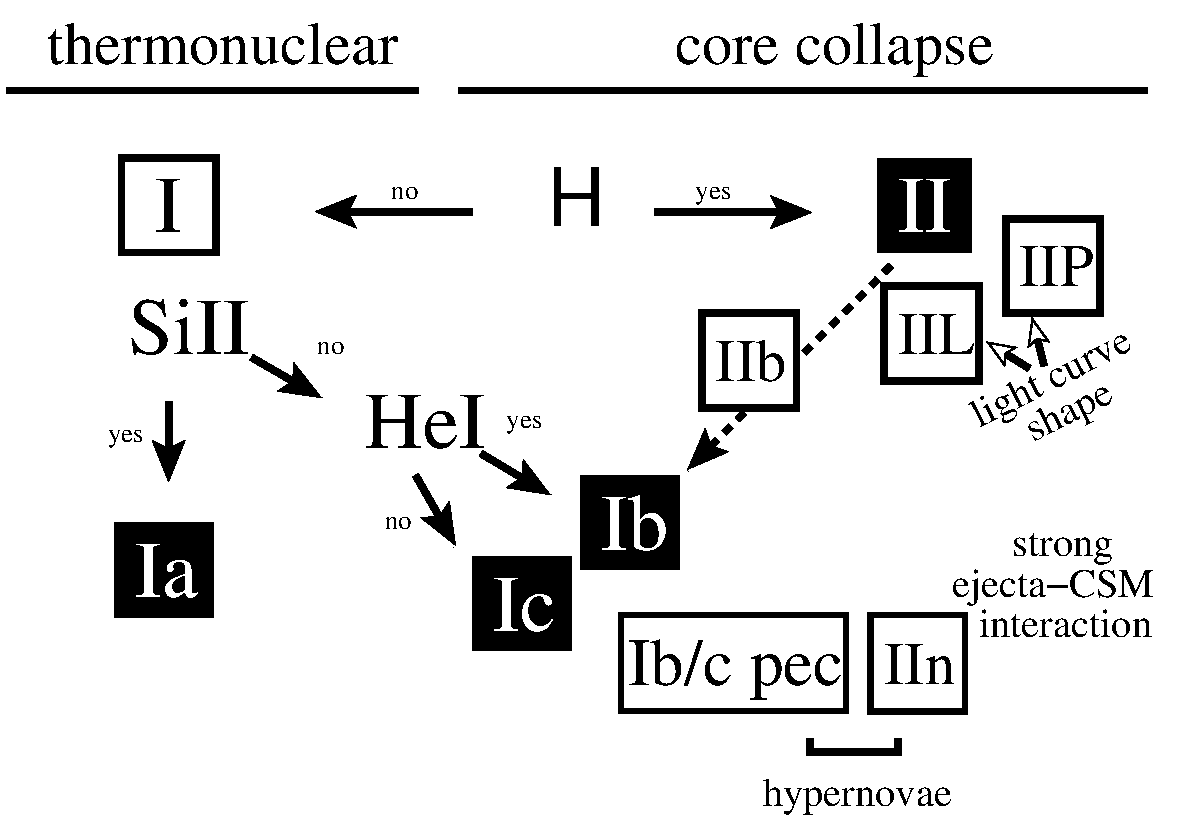
\includegraphics[width=\textwidth]{chapter1/plots/sn_classification.pdf} 
   \caption{}
   \label{fig:sn_classification}
\end{figure}

This basic classification has remained to this day, however the two main classes branched into several subtypes.
During the 1980s the community discovered that most \sneia\ showed a broad Si II line at 6130 \AA, but that there was a distinct subclass of objects that lacked this feature. These Silicon-less objects were then subclassed further into objects that showed helium -- now known as Type Ib --  and those that did not were called Type Ic \citep{1987ApJ...317..355H, 1986ApJ...306L..77G}. The classical Type I supernova was renamed to Type Ia (see Figure \ref{fig:sn_classification}). 

\begin{figure}[htbp] %  figure placement: here, top, bottom, or page
   \centering
   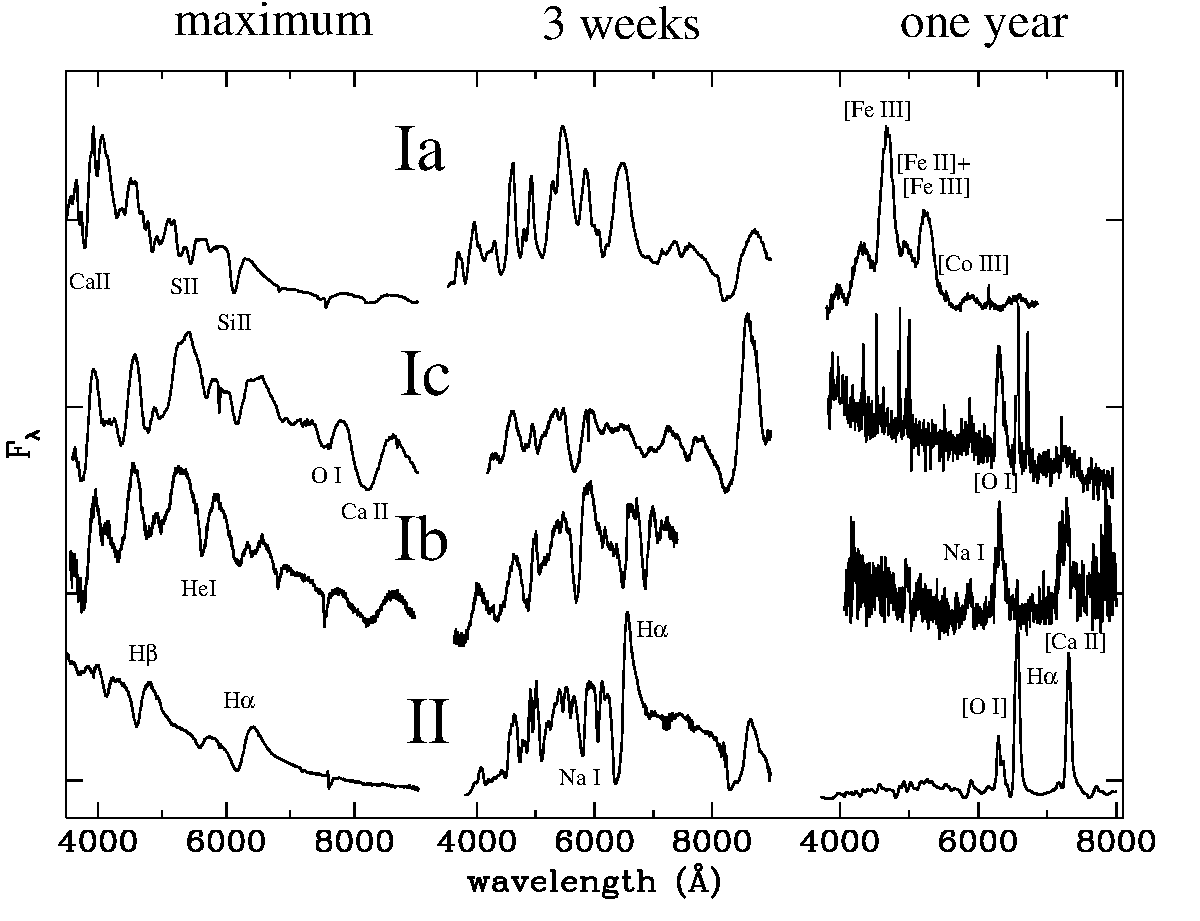
\includegraphics[width=\textwidth]{chapter1/plots/sn_class_spectra.pdf} 
   \caption{example caption}
   \label{fig:sn_class_spectra}
\end{figure}

This classification only uses static spectral features. In recent years, however, there has been a push towards also using the lightcurve and spectral evolution as classification parameters. \citet{2005ApJ...623.1011B} provide an overview of this subclassing of \sneia\ and suggest that there are two distinct subclasses of \sneia. As a parameter for this further partitioning they use the velocity measured from the Si II feature at 6355 \AA. Those with a relatively fast decline in this radial velocity they call \hvg\ (high velocity gradient) those with a slow decline rate are named \lvg\ (low velocity gradient). 
Figure \ref{fig:sn_class_lvg_hvg} shows the velocity gradient of 26 supernovae taken from  \citet{2005ApJ...623.1011B}

\begin{figure}[htbp] %  figure placement: here, top, bottom, or page
   \centering
   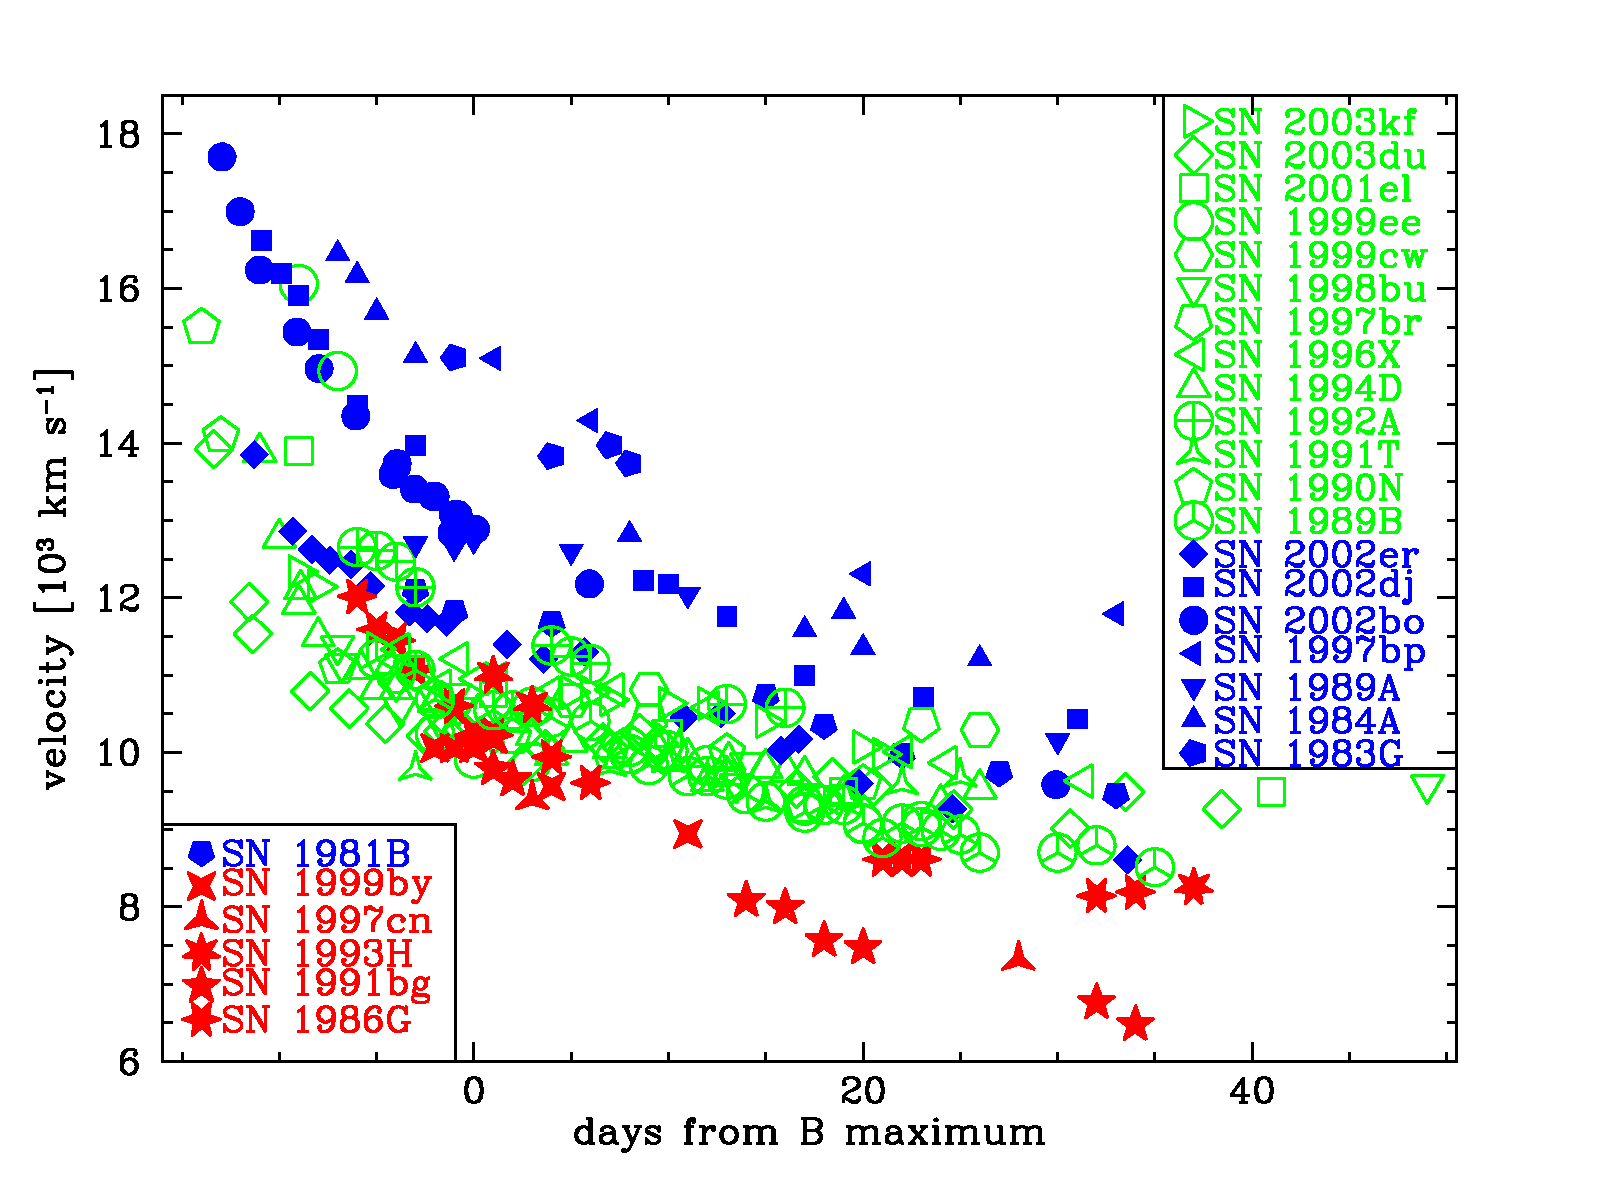
\includegraphics[width=\textwidth]{chapter1/plots/velocity_gradient.pdf} 
   \caption{example caption}
   \label{fig:sn_class_lvg_hvg}
\end{figure}

Futhermore there seems to be also a split in the intrinsic luminosity of \sneia. The canonical objects for these distinct brightness classes are the overluminous 1991T \citet{1992AJ....103.1632P} and the faint 1991bg .
Faint supernovae are fast decliners both in velocity as well as luminosity \citet{2005ApJ...623.1011B}. The bright supernovae seem to occur in both the \hvg\ and \lvg\ group. I will discuss the physical implications of these two subtypes in section \ref{sec:snia_physics}.

In summary, although there are several different subclasses the \snia as a class itself is relatively homogenous when compared to the different \sneii. ??? rates????


\sneii span large ranges in observables like luminosity, explosion energies, etc. We can divide the main class into three main subclasses Type II Plateau \citet[\sniip][]{1979A&A....72..287B} which have a relatively flat lightcurve after an initial maximum, in contrast the Type II Linear \cite[\sniil][]{1990MNRAS.244..269S} has a rapid linear decline after the maximum. The third subclass is the narrow-lined \snii (\sniin) which is characterized by narrow emission lines, which are thought to come from interaction with the \csm. Unlike the \sneia there are numerous intermediate objects among these three basic classes. 

???? 

For a more comprehensive review of the classification of supernovae the reader should consult \citet{2003LNP...598...21T, 2007AIPC..937..187T}.

\section{Type II Supernova}
\subsection{Observation}

\subsection{Theory}


nucelosynthesis
first stars
hypernovae
GRB connection
massive stars
expanding photosphere -> distance measurements
binary evoltion

\section{Type Ib/c Supernova}


\section{Type Ia Supernova}
binary evolution
chandrasekhar
white dwarfs
nucleosynthesis
iron in particular

cosmology

\section{Progenitors of Type Ia progenitors}
\label{sec:snia_progenitor}



% !TEX root =../thesis.tex
\chapter{SN1572}
\label{chap:SN1572}

\section{Introduction}
Type Ia supernovae (SNe Ia) are of broad interest. They serve as
physically interesting end points of stellar evolution, are major
contributors to galactic chemical evolution, and serve as one of
astronomy's most powerful cosmological tools.

It is therefore unfortunate that the identity of the progenitors
of SNe Ia is still uncertain. For example, without knowing the progenitors,
the time scales of SNe Ia enriching the interstellar medium with iron
remains highly uncertain. But it is the crippling impact on the
cosmological application of these objects which is especially
profound; it is impossible to predict the consequences of any
cosmological evolution of these objects or even gauge the likelihood of
such evolution occurring.

There is broad agreement that the stars which explode as SNe Ia are
white dwarfs which have accreted material in a binary system until
they are near the Chandrasekhar mass, then start to ignite carbon
explosively, which leads to a thermonuclear detonation/deflagration of the
star. It is the identity of the binary companion that is currently
completely undetermined. Suggestions fall into two general categories
\citep{1997thsu.conf..111I}:
\begin{itemize}
\item Single degenerate systems in which a white dwarf accretes mass
from a non-degenerate companion, where the companion could be a
main-sequence star, a subgiant, a red giant, or possibly even a
subdwarf.
\item Double degenerate systems where two CO white dwarfs merge,
resulting in a single object with a mass above the Chandrasekhar limit.
\end{itemize}

The detection of circumstellar material around SN~2006X
\citep{2007Sci...317..924P} has provided support for the single
degenerate model in this case, although the lack of substantial 
hydrogen in several other SNe Ia \citep{2007ApJ...670.1275L} 
poses more of a challenge to this scenario.

These models also make different predictions for the nature of the system
following the explosion. In the double degenerate case, no stellar
object remains, but for a single white dwarf, the binary
companion remains largely intact.

In the single degenerate case, the expected effect of the SN on the
donor star has been investigated by \citet*{2000ApJS..128..615M}, who
have calculated the impact of a SN Ia explosion on a variety of binary
companions. \citet*{2001ApJ...550L..53C} have explored many of the
observational consequences of the possible scenarios, and
Podsiadlowski (2003) has presented models that follow both the
pre-supernova accretion phase and the post-explosion non-equilibrium
evolution of the companion star that has been strongly perturbed by
the impact of the supernova shell.  To summarize these results,
main-sequence and subgiant companions lose 10\,--\,20 \% of their
envelopes and have a resulting space velocity of 180\,--\,320\,\kms . Red-giant companions lose most of its hydrogen envelope, leaving a
helium core with a small amount of hydrogen-rich envelope material behind,
and acquire a space velocity of about 10\,--\,100\,\kms.
\citet{2008A&A...489..943P} have used a binary stellar evolution code on a main-sequence star and exposed the evolved star to a SN Ia. Their simulations show that even less material is stripped due to the compact nature of a star that evolved in a binary. We will use their results where applicable. 

\citet[henceforth \rl]{2004Natur.431.1069R} have identified what might
be the donor star to Tycho's SN, a SN Ia which exploded in the Milky
Way in 1572. These authors presented evidence that this star, \starg\
by their naming convention, is at a distance consistent with the Tycho
supernova remnant (henceforth SNR), has a significant peculiar radial
velocity and proper motion, roughly solar abundance, and a surface
gravity lower than a main-sequence star. However, \starg\ is located at a significant distance from the
inferred center of the remnant, and any process that has displaced the
star must preserve the remnant's nearly perfectly circular projected shape. During the final stages of refereeing of this paper we were made aware of the article by \citet[henceforth \gh]{2009ApJ...691....1H}, who used Keck HIRES data to better constrain \starg's stellar parameters, and in addition, found an enhancement in Nickel abundance, relative to normal metal rich stars.

\citet{2007PASJ...59..811I} have looked for Fe absorption lines from
the remnant, using nearby stars as continuum sources, with the hope to
better constrain the distance of these stars to the SNR. With their technique, stars in the
remnant's center should show strong blue-shifted Fe absorption lines,
formed by material in the expanding shell of Fe-rich material from the
SN, moving towards the observer.  Stars in the foreground would show
no Fe absorption, and background stars both red- and blue-shifted
absorption. Their study shows that \starg\ does not contain any
significant blue-shifted Fe absorption lines, suggesting that \starg\
is in the remnant's foreground. However, these observations and their
analysis, while suggestive, cannot be considered a conclusive rebuttal
of \starg's association with the remnant; this technique requires a significant column depth of Fe which is not guaranteed. A lack of Fe column depth may be indicated by the fact that no stars were found in the
vicinity of the remnant that showed both blue- and red-shifted absorption lines.

To further examine the \rl\ suggested association of \starg\ with the
SN Ia progenitor, we have obtained a high-resolution spectrum of the
star using Subaru and its High Dispersion Spectrograph
\citep{1998SPIE.3355..354N}.

We summarize, in section 2, the observational
circumstances of the Tycho remnant and any donor star, and argue in
section 3 that rapid rotation is an important, previously unrealised
signature in a SN Ia donor star. In section 4 we describe our
Subaru observations. Section 5 covers the analysis of data and the results of this analysis. Section 6 compares the relative merit for \starg\ being the donor star to the
Tycho SN or being an unrelated background star, and in section 7 we summarize our findings and motivate future observations.

\section{Observational Characteristics of the Tycho Remnant and Star-G}

\rl\ have done a thorough job summarizing the relevant details of the
Tycho remnant. The remnant shows the characteristics expected of a SN
Ia based on its light curve (measured by Tycho Brahe himself),
chemical abundances, and current X-ray and radio emission
\citep{2004ApJ...612..357R}. In figure \ref{fig:overview} we have overlaid radio contours\footnote{The National Radio Astronomy Observatory is a facility of the National Science Foundation operated under cooperative agreement by Associated Universities, Inc.}  on an optical image and have marked the position of the stars mentioned in this and \rl's work.


\begin{figure}[h!]
\includegraphics*[width = \textwidth]{chapter2/plots/overview.pdf}
\caption{Radio Contours (VLA Project AM0347) have been overlaid \citep{1996ASPC..101...80G} on an R-Band Image (NGS-POSS). The cutout is an INT image (see text). The stars marked in the figure are mentioned in this work and in \rl's work. }
\label{fig:overview}
\end{figure}

Although it is not easy to measure the
remnant's distance precisely, \rl\ estimated Tycho's SNR distance to be $2.8 \pm 0.8$\,kpc, using the ratio of the SN 1006 and Tycho SNR's angular sizes and their relative ages, and the direct distance measure of SN 1006 by \citeauthor*{2003ApJ...585..324W} (2003).  \citet{2008Natur.456..617K} have recently shown, from a spectrum of a light echo associated with the SN1572, that this SN was a normal SN Ia. Using Tycho's observed light curve, the properties of SN Ia as standard candles, and an extinction value they find a distance to the SN of $3.8^{+1.5}_{-1.1}$\,kpc. Updating their values for the extinction values determined in this paper (section \ref{sec:distmod}), as well as using an absolute magnitude for SN Ia of $-19.5 \pm 0.25$ \citep{2004MNRAS.349.1344A}, we find a distance of $3.4^{+1.3}_{-1.0}$\,kpc. In summary, we believe the remnant's distance is poorly constrained, but probably between 2 and 4.5\,kpc.
\label{sec:obschar}
\rl\ also report the
spectroscopic and photometric properties for the bright stars near the
center of the Tycho remnant and find a uniform value of approximately
$E(B-V)=0.6$ for stars more distant than 2 kpc. \gh\ have revised the $E(B-V)$ value for \starg\ to 0.76.

In addition, for a select list of stars, \rl\ provide radial velocities and proper
motions. 
For \starg, \rl\ report a value of $v_r=-99\pm6$\,\kms\ for
the radial velocity in the Local Standard of Rest (henceforth LSR), a
proper motion of $\mu_b=-6.1 \pm 1.3$\,\masyr, $\mu_l=-2.6 \pm
1.3$\,\masyr, $\log{g} = 3.5 \pm 0.5$, and $T=5750$\,K.  Using HIRES data \gh\ have improved the measurements of \starg's stellar parameters, finding  $v_r \approx -80$\,\kms, $\log{g} = 3.85 \pm 0.3$, $T=5900 \pm 100$\,K, and $\rm{[Fe/H]}=-0.05 \pm 0.09$\,dex. We note that
\citet{2007PASJ...59..811I} have classified \starg\ as an F8V star ($T
\approx 6250 $\,K, $\log{g} \approx 4.3$,
\citealt{1982lbor.book.....A}), in significant disagreement with the
\rl\ temperature and gravity. We believe the \gh\  values are based on by far the best data, and for the purpose of this paper, we will adopt their values. 

Based on the observations, \rl\ asserted that \starg\ was located at
approximately $3\pm 0.5$\,kpc -- consistent with the remnant's
distance.  They note that this star has solar
metallicity, and therefore its kinematic signature was not
attributable to being a member of the Galactic halo. 
They further argued that \starg's radial velocity and proper
motion were both inconsistent with the distance, a simple Galactic
rotation model, and the star being part of the disk population of the Milky Way.
 The derived physical characteristics of the system were nearly identical to
what was proposed by Podsiadlowski (2003) for a typical SN Ia donor
star emerging from a single degenerate system \citep[e.g., U Sco; also see ][]{Hachisu:1996p758,Li:1997p437,Hachisu:1999p431,Han:2004p444,Han:2008p726}. The revision in the stellar parameters by
\gh\ leads to different distance with a larger uncertainty, but by and large, has not altered the conclusions above. Taken in total, the data provide a rather convincing case for the association of \starg\ with the Tycho SN.

\section{Rapid Rotation: A Key Signature in SN Ia Donor Stars}
\label{sec:rot}
In the single degenerate SN Ia progenitor channel, mass is transferred
at a high rate from a secondary star onto a white dwarf \citep{Nomoto:1982p451,Nomoto:2007p480}. These high
mass-transfer rates require that the secondary star overflows its
Roche lobe. Due to the strong tidal coupling of a Roche-lobe filling
donor, the secondary is expected to be tidally locked to the orbit
(i.e., have the same rotation period as the orbital period).  At the
time of the SN explosion, the donor star is released from its orbit, but
will continue with the same space velocity as its former orbital
velocity and continue to rotate at its tidally induced rate.

\begin{figure}[h!]
\centering
\includegraphics*[width=\textwidth]{chapter2/plots/theo_rot_podsi.pdf}
\caption{The expected rotation rate for a donor star as a function of
its mass at the time of the explosion. The three curves show the results for 3 final space
velocities of the donor star (similar to those suggested by RP04). It
is assumed that the white dwarf has a mass of 1.4\,$M_\odot$.}
\label{fig:theorot}
\end{figure}

There is a simple relationship between the secondary's rotation
velocity $(v_{\rm orb, 2})$ and its orbital velocity:

$$ v_{\rm rot} = {M_1 + M_2\over M_1}\,f(q)\,v_{\rm orb, 2} ,$$

where $f(q)$ is the ratio of the secondary's Roche-lobe radius to the
orbital separation \citep[e.g., given by][]{1983ApJ...268..368E} and
$q=M_1/M_2$ is the mass ratio of the components at the time of the
explosion. Figure \ref{fig:theorot} shows the rotational velocity as a
function of secondary mass for several values of $v_{\rm orb, 2}$ (consistent with \rl s measurement, and at the low end of values expected for a subgiant star),
where we assumed that the exploding white dwarf had a mass of
$1.4\,M_\odot$.

This estimate is strictly speaking an upper limit, as it does not
take into account the angular-momentum loss associated with the
stripping of envelope material by the supernova and any bloating due
to the supernova heating. The latter would reduce the rotational
velocity to first order by a factor equal to the bloating
factor (i.e. the ratio of the new to the old radius), but the
star would likely find itself in a state where its radius and
temperature was atypical of a normal star. 

According to the results of  \citet{2000ApJS..128..615M}, mass stripping is
not likely to be significant if the companion is a main-sequence star
or a subgiant. Furthermore, following binary evolution of a main-sequence star, \citet{2008A&A...489..943P} have shown that even less material is stripped. However, if the companion is a giant, it would be
stripped of most of its envelope.  Such a star would not show any
signs of rapid rotation since the initial giant would have been
relatively slowly rotating; e.g., if one assumes solid-body rotation
in the envelope, the rotation velocity at $\sim 1\, R_\odot$ will only
be $\sim 0.5\,$km\,s$^{-1}$ for a pre-SN orbital period of
100\,d. Moreover, the material at the surface may have expanded from
its original radius inside the giant, further reducing the rotational
velocity. However, if the stripping is less than estimated by  \citet{2000ApJS..128..615M}, then it is possible for the signature of rotation to persist for a giant, albeit at a much lower velocity.

 \citet{2000ApJS..128..615M} also showed that due to the interaction
of the SN blast wave with the companion, the secondary may receive
a moderate kick of up to a few 10\,km\,s$^{-1}$, but this kick
is generally much lower than $v_{\rm orb,2}$ and therefore does
not significantly affect the resulting space velocity.

Finally, we note that the observed rotation velocities are reduced by
a factor $\sin i$, where $i$ is the inclination angle.  However,
because the donor star's rotational axis can be assumed to be parallel
to its orbital axis, a minimum observed rotation speed can be computed
from the observed peculiar radial velocity (observed radial velocity
minus the expected radial velocity of an object at that distance and
direction). It is only if the orbital motion (and hence final systemic
velocity) is solely in the plane of the sky, that $\sin{i}$, and
therefore, the observed rotation, approaches
zero.\label{rotation_expl}

\section{Subaru Observations}
To investigate the rotational properties of \starg, we were granted time
with the Subaru telescope. Our observations of \starg\ were taken in
service mode on the nights of 2005 10 17 and 2005 10 18. 9
spectra were taken with the High Dispersion Spectrograph
\citep[HDS, ][]{1998SPIE.3355..354N} with a resolution of $\rm{R}\simeq40000$ (measured using the instrumental broadening of the Thorium-Argon arc lines), an
exposure time of 2000 seconds each (totalling to 5 hours) and a signal to noise ratio of about 10 per pixel (measured at $8300$\,\AA\ with 0.1 \AA\,pixel$^{-1}$) . The HDS
features two arms, with each arm feeding a 2-chip CCD mosaic. The blue
arm covers 6170\,\AA\ to 7402\,\AA\ and the red arm 7594\,\AA\ to
8818\,\AA. An OG530 filter was used to block contamination from light
blueward of our observing window, and data were binned by 4 in both
the spatial and spectral directions, resulting in a pixel size of
0.1\,\AA\ (at 8000\,\AA) by 0.55$^{\prime\prime}$.

Data were pre-processed using tools provided by the HDS team and then
bias-subtracted. We created a mask from bias and flatfielded frames,
where we isolated the echelle orders and flagged bad pixel
regions. The data were flatfielded using internal quartz flats, and the
2-D images cleaned of cosmic rays (and checked carefully by eye to
ensure there were no unintended consequences) using an algorithm
supplied by M. Ashley (private communication). The spectrum of each
echelle order was extracted using IRAF\footnote{IRAF is distributed by
the National Optical Astronomy Observatory, which is operated by the
Association of Universities for Research in Astronomy (AURA) under
cooperative agreement with the National Science Foundation.}  echelle
routines, with wavelength calibrations based around low-order fits of
a Thorium-Argon arc. Wavelength calibration of each extracted spectrum
was checked against atmospheric O$_2$, and our solutions were found to
be accurate in all cases to within 1\,\kms\
\citep{1985A&A...149..357C}. Unfortunately, we lacked a smooth
spectrum standard star for setting the continuum, and we resorted to
calculating a median of the spectra (6\,\AA\ window) and dividing the
spectra through this smoothed median. This unusual method was chosen
over the common approach of fitting the spectrum with a polynomial,
due to the special characteristics of this observation (low signal to noise ratio, and a complex instrumental response). While this does not affect the narrow lines our program was
targetting, it does affect broad lines such as the H$\alpha$ and the
CaII IR triplet. The final step was to combine all spectra and remove
any remaining cosmic rays (in the 1D spectra) by hand.

\section{Analysis and Results}

\subsection{Rotational measurement}

To attain the rotational velocity of the candidate star, we measured
several unblended and strong (but not saturated) Fe I lines in the
spectrum \citep{1974lafl.book.....W}. Since our spectrum only had a
combined signal to noise ratio of approximately 10, we added the
spectra of the lines after normalizing them to the same equivalent
width. As a reference we created three synthetic spectra (one broadened only with the instrumental profile, the others with the instrumental profile and $v_{\rm{rot}}\sin{i}$ of 10 and 15\,\kms\ respectively) with the 2007 version of MOOG \citep{1973ApJ...184..839S}, using \gh's temperature, gravity and metallicity.  We use a standard value of $\beta=3/2$ for the limb darkening although the choice
of this value is not critical, which we confirmed by checking our
results using significantly different values of $\beta$. Figure
\ref{fig:sunobjrot} shows the comparison between the synthetic spectra of different rotational velocity and the spectrum of \starg. We have scaled the synthetic spectrum using the equivalent width. This comparison indicates that the stellar broadening (rotational, macro turbulence, etc. ) is less than broadening due to the instrumental profile of 7.5\,\kms, and therefore we adopt 7.5\,\kms\ as our upper limit to the rotation of the star. If one were to adopt \rl's measurements of the
peculiar spatial motion, it could be concluded that $\sin{i}$ is much closer
to 1 than 0 (see the end of section \ref{rotation_expl} for further
explanation) and thus that the rotational speed is $v_{\rm rot} \lesssim 7.5$\,\kms.

\begin{figure}[h!]
\centering
\includegraphics*[width=0.45\textwidth]{chapter2/plots/precombobj_sn1572.pdf}
\includegraphics*[width=0.45\textwidth]{chapter2/plots/rotcomp_subaru_starg.pdf}
\caption{Six observed Fe I line profiles of  \starg\ are shown on the left panel. The right panel shows the combination of these line profiles after normalization to the same equivalent width and compares them to the spectrum of the Sun, which is convolved with 3 different values for the rotational broadening kernel. \starg\ does not show significant rotation, indicating $v_{\rm{rot}} \sin{i} \lesssim 7.5$\,\kms.}
\label{fig:sunobjrot}
\end{figure}

\subsection{Radial velocity}

To determine the radial velocity, we used 63 lines to measure the shift
in wavelength. We find a radial velocity in the topocentric (Mauna
Kea) frame of reference of $v_{\rm top} = - 92.7 \pm 0.2$\,\kms (the
error being the standard deviation of 63 measurements) . The
conversion from the topocentric to the Galactic LSR for our
observations was calculated to be 13.6 \kms\ (IRAF task rvcorrect)
using the IAU standard of motion. Including the uncertainty in the LSR
definition, we find a radial velocity in the LSR for \starg\ of
$v_{\rm LSR} = -79 \pm 2$\,\kms. This is in significant disagreement
with that reported by \rl, but agrees with the revised value published by \gh.


\subsection{Astrometry}
\rl\ have measured a significant proper motion for \starg\ of $\mu_b=-6.1 \pm 1.3$ \masyr, $\mu_l=-2.6 \pm 1.3$\ \masyr. Because \starg\ is metal rich, and at a distance of $D>2$kpc, this measurement provides one of the strongest arguments for \starg\ being the donor star to Tycho SN. It is almost impossible to account for this proper motion, equivalent to a $v_b=58\left({{D}\over{2\rm{~kpc}}}\right)$\kms\ or 3 times the disk's velocity dispersion of $\sigma_z=19$\kms, except through some sort of strong binary star interaction.  

However, the \hst\ data present an especially difficult set of issues in obtaining astrometry free of systematic errors. For \starg\ these issues include the PSF on the first epoch WFPC2 image being grossly undersampled, both the ACS and WFPC2 focal planes being highly distorted,  poor and different charge transfer efficiency across the two \hst\ images, and that \starg\ was, unfortunately, located at the edge of one of the WFPC2 chips, making it especially difficult to understand the errors associated with it. Smaller issues include the small field of overlap between the two images, making the measurement subject to issues of the correlated motions of stars, especially in the $\mu_l$ direction.

To cross-check \rl's proper motion of Star-G , we have scanned a photographic plate taken in
September 1970 on the Palomar 5 meter, and compared this to an Isaac
Newton 2.5\,m Telescope (INT) CCD archive image (INT200408090414934) of the remnant taken in
August 2004. The Palomar plate has an image FWHM of $1.7^{\prime\prime}$, and the INT image $0.88^{\prime\prime}$. While our images have a much larger PSF than the HST images, the images have significantly less distortion, are matched over a larger field of view with more stars, have fully sampled PSFs, and were taken across nearly an 8 times longer time baseline. The photographic nature of the first epoch does add complications not present in the \hst\ data. The non-linear response of photographic plates causes their astrometry to have systematic effects as a function of brightness \citep{2001ASPC..232..311C}, especially affecting objects near the plate limit, where  single grains are largely responsible for the detection of an object. 


The position of stars on the INT image were matched to
the 2MASS point source catalog \citep{2006AJ....131.1163S} to get a coordinate 
transformation (pixel coordinates to celestial coordinates) using a
3rd-order polynomial fit with an RMS precision of 40 mas with 180 stars. This fit is limited by precision of the 2MASS catalog and shows no systematic residuals as a function of magnitude, or position.  Using this  world coordinate system (WCS) transformation, we then derived the
positions of all stars on the INT image. The coordinates of 60 uncrowded
stars on the Palomar plate were matched to the INT-based catalog, and a 3rd-order polynomial was used to transform the Palomar positions to the INT-based positions. The fit has an RMS of 65 mas in the direction of galactic longitude, and 45mas in the direction of galactic latitude.  We believe the larger scatter in the direction of  Galactic longitude is due to the shape of the PSF being slightly non-symmetric in the direction of tracking on the Palomar plate. This tracking (in RA, which is close to the direction of galactic longitude), causes the position of stars to depend slightly on their brightness. This explanation is supported by  a small systematic trend in our astrometric data in $\mu_l$, not seen in $\mu_b$, as a function of $m_R$.  An alternative explanation is that the  trend in $\mu_l$ is caused by the average motion of stars changing due to galactic rotation as a function of distance, which is proxied by $m_R$.  We have used the Besan\c{c}on Galactic model \citep{2003A&A...409..523R} to estimate the size of any such effect, and find the observed effect is an order of magnitude larger than what is expected. The systemic difference between assuming either source of the observed effect is less than 1\,\masyr\ in $\mu_l$, and has no effect in our $\mu_b$ measurement. In our final proper motions, presented in table \ref{tab:prop_motion}, we remove  the systematic trend as a function of $m_R$ with a linear function.

\begin{table}[htbp]
\caption{Proper motions of stars within $45^{\prime\prime}$ of the Tycho SNR center.}
\begin{tabular}{ccccccc}
\hline\hline														
$\alpha$ &	$\delta$	&	$\mu_l$	&	$\mu_b$	&	$m_R$	&	$\theta$ \\		
\,[hh:mm:ss.ss] & [dd:mm:ss.ss] & [\masyr] & [\masyr] & [mag] & [arcsec] & Name \\
%RA                                     & DEC                                      & Proper motion in $l$      &      Proper motion in $b$ &   apparent magnitude in R (\rl) & distance from center & designation given by \rl \\
\hline
														
00:25:20.40	&	+64:08:12.32	&	-0.90	&	-0.56	&	17.05	&	08.9	&	c	\\	
00:25:18.29	&	+64:08:16.12	&	-4.25	&	-0.81	&	18.80	&	10.0	&	e	\\	
00:25:17.10	&	+64:08:30.99	&	-1.82	&	1.78	&	16.87	&	20.3	&	f	\\	
00:25:23.58	&	+64:08:02.02	&	-1.58	&	-2.71	&	17.83	&	31.1	&	g	\\	
00:25:15.52	&	+64:08:35.44	&	1.94	&	0.83	&	20.28	&	31.4	&	r	\\	
00:25:15.08	&	+64:08:05.95	&	-0.67	&	1.49	&	18.86	&	33.3	&	j	\\	
00:25:23.89	&	+64:08:39.33	&	-0.31	&	1.08	&	19.20	&	33.5	&	k	\\	
00:25:14.74	&	+64:08:28.16	&	2.60	&	1.46	&	17.45	&	33.5	&	n	\\	
00:25:14.81	&	+64:08:34.22	&	4.05	&	-2.05	&	19.35	&	35.0	&	q	\\	
00:25:13.79	&	+64:08:34.50	&	2.32	&	1.01	&	19.90	&	41.3	&	s	\\	
00:25:14.59	&	+64:07:55.10	&	-3.94	&	2.35	&	19.23	&	41.7	&	t	\\	
00:25:19.25	&	+64:07:38.00	&	1.75	&	-3.43	&	16.86	&	42.1	&	u	\\	
00:25:22.45	&	+64:07:32.49	&	81.29	&	-2.68	&	19.81	&	48.7	&	HP-1	\\	\hline

\end{tabular}
\label{tab:prop_motion}

\end{table}

To measure the proper motion of each star, we exclude each star from the astrometric transformation fit
so as not to bias its proper motion measurement.  Comparing the stellar positions in the 34 year interval we find that these 60 stars show an RMS dispersion  $\sigma_{\mu_l} = 2.1$\masyr, $\sigma_{\mu_b} =1.6$\,\masyr. For
\starg\ we measure $\mu_l = -1.6 \pm 2.1$\,\masyr, $\mu_b = -2.7 \pm 1.6$\,\masyr; this implies that no significant proper motion is detected. We do note that this measurement has a similar precision to
that of \rl, is consistent with no observed motion, and is in moderate disagreement with the \rl\ measurement.

\begin{figure}[h!]
	\centering
	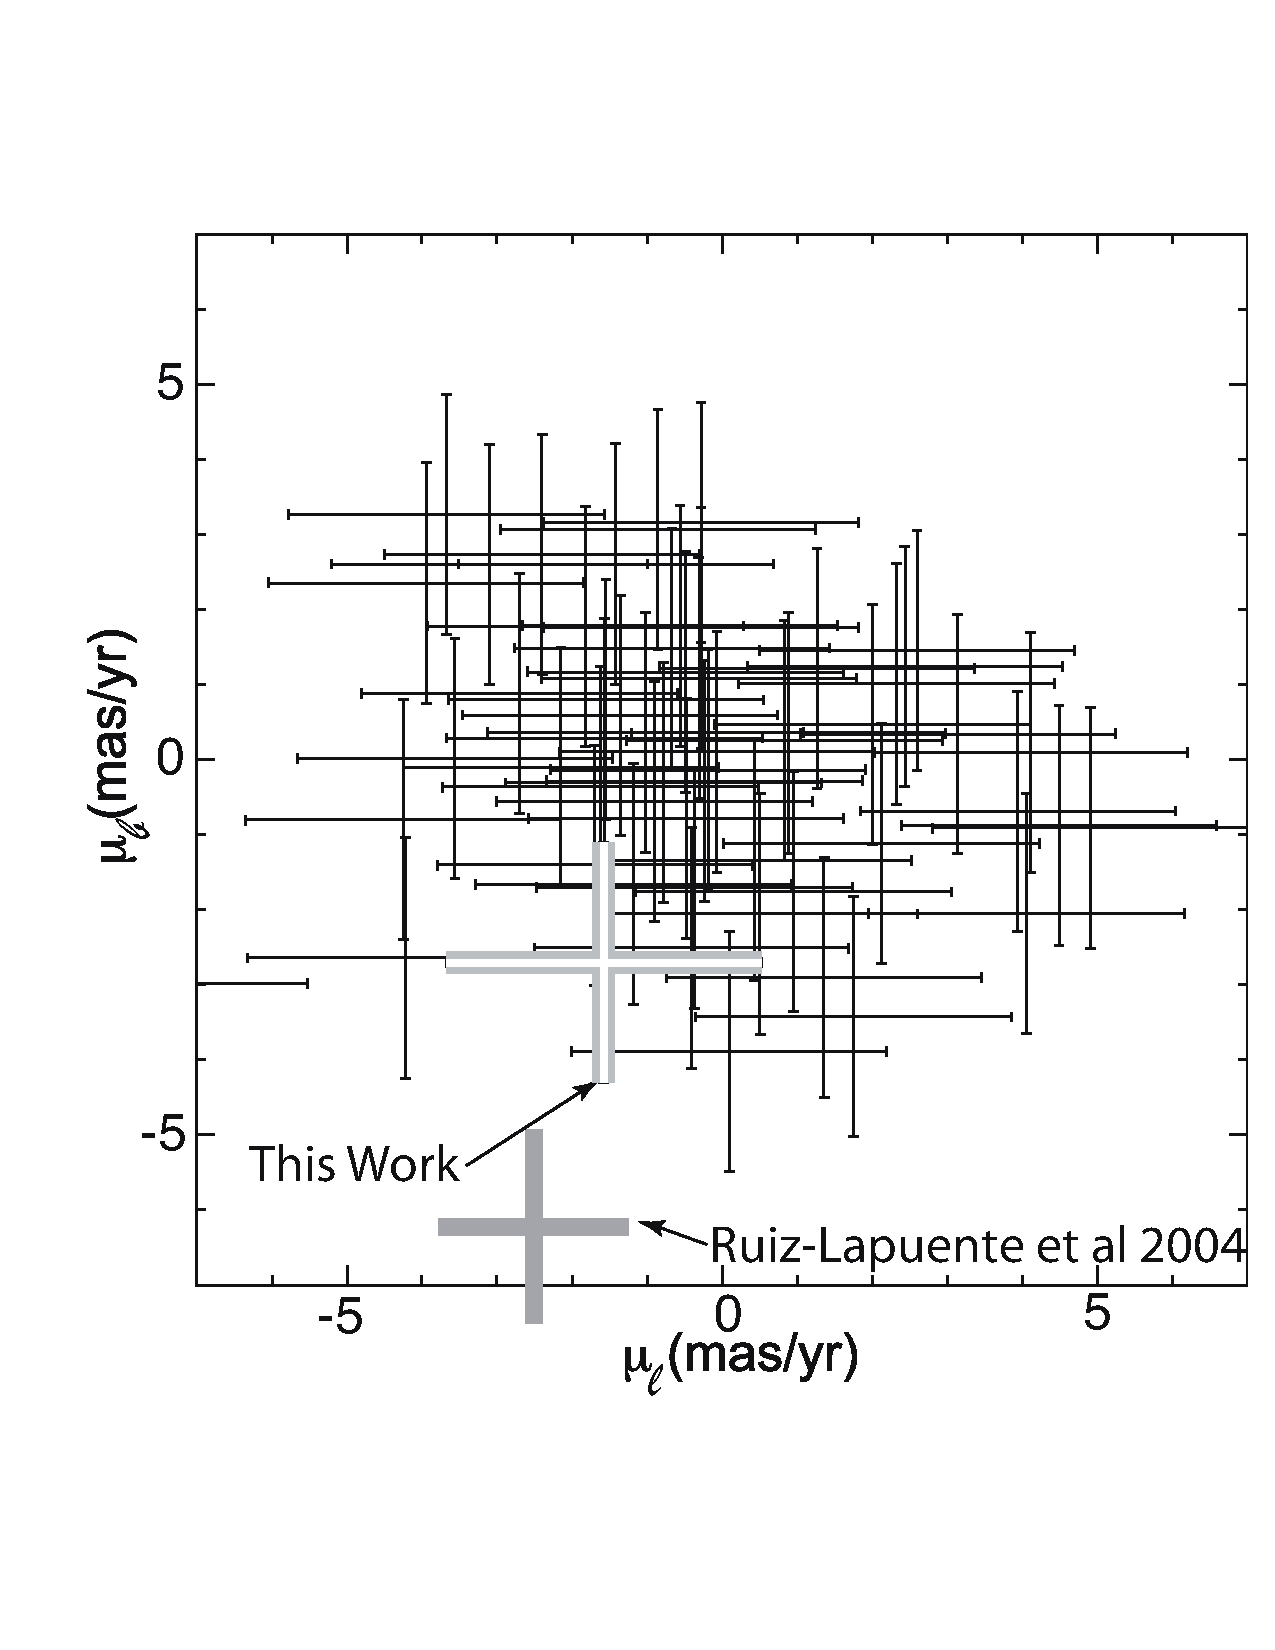
\includegraphics[width=\textwidth]{chapter2/plots/prop_motion_compare_subaru.pdf}
\caption{The astrometric motions of 60 stars measured in the Tycho SNR
center. The measurements have a RMS dispersion of 1.6\,\masyr. Shown
in grey is the proper motion of \starg\ measured here and by RP04, showing a moderate discrepancy in the two measurements. Our measurement is consistent with no proper motion. }
\label{fig:prop_motion}
\end{figure}

In table \ref{tab:prop_motion} we present our astrometric measurements of all stars listed by \rl\  for which we were able to measure proper motions. We also give the apparent magnitudes in R (partly measured by this work and partly by \rl) and the distance from center $\theta$. Due to crowding caused by the relatively poor resolution of the first epoch photographic plate, several stars are not included that could be measured using \hst.
We include an  additional star, not cataloged by \rl, which exhibits high proper motion. This  high proper motion star, which was off the WFPC2 images of \rl,  we designate HP-1, and has a proper motion of $\mu_l=81.3$, $\mu_b=-2.7$ \masyr. Due to the distance from the remnant's center, (we estimate HP-1 would have been located 51$^{\prime\prime}$ from the remnant's center in 1572), we doubt this star is connected to the Tycho SN, but we include it for the sake of completeness. 

\section{Discussion}


\subsection{A Background interloper?}
A previously unrecognized property for many progenitor scenarios is the rapid post-explosion rotation of the donor (as described in section \ref{sec:rot}).
The expected rotation as calculated in Figure \ref{fig:theorot} is
large compared to that expected of stars with a spectral type later
than F and should be easily observable. We have shown \starg's rotation to be less ($v_{\rm rot} \sin{i} \lesssim 7.5 $\,\kms) than what is expected  of an associated star if the companion was a main-sequence star or subgiant. A red giant scenario where the envelope's bloating has significantly decreased rotation could be consistent with our observation of \starg, and this will be discussed in section \ref{redgiant}.

The primary basis for which \rl\ selected \starg\ as a candidate for
the donor star to the Tycho SN was the combination of its large peculiar radial velocity
and its observed proper motion. In Figure \ref{fig:bes_d_mu} we
use the Besan\c{c}on Galactic model \citep{2003A&A...409..523R} to
construct an expected set of radial velocities for metal-rich stars in the
direction of SN1572.

\begin{figure}[htb!]
\centering
\includegraphics* [scale=0.5,angle=0]{chapter2/plots/sn1572_d_vr_subaru.pdf}
\caption{Besan\c{c}on model for a metal rich ([Fe/H] $>$ -0.2 ) Galactic population between 0 and 7\,kpc in the direction of Tycho SNR (l = 120.1, b=1.4) with a solid angle of 1 square degree.
The remnant's distance is represented by the black dashed lines (as calculated in section \ref{sec:obschar}). The contours show the radial velocity distribution. 
Our measured radial velocity corrected to LSR and our distance are shown, with their respective error ranges, as the black rectangle.  The distance  range calculated by \gh\ are indicated by the two solid lines. The observed LSR $v_r$ for \starg\ is mildly unusual for stars at the remnant's distance, and is consistent with the bulk of stars behind
the remnant. }
\label{fig:bes_d_mu}
\end{figure}

Measuring the distance to \starg\ is a key discriminant in associating the star to the SN explosion. To improve the uncertainty of the distance to the star, due both to temperature and extinction uncertainty,  we base our distance on the observed $m_K$ \citep{2006AJ....131.1163S} and ($V-K$) color (\rl).  We interpolate ATLAS9 models without overshoot \citep*{1998A&A...333..231B} to find a theoretical $V-K$ and absolute magnitude for the \gh's values of temperature and gravity. Using a standard extinction law \citep*{1989ApJ...345..245C} ($A_V= 3.12 E(B-V)$ and $A_K/A_V=0.109$) to match the theoretical and observed colors, we find $A_V=2.58\pm0.08$mag, $A_K=0.28\pm 0.01$ mag, and $E(B-V)=0.84\pm0.05$.  To better show the uncertainties, we present our distance moduli scaled to the observed and derived values of extinction, temperature and gravity.
The temperature coefficients were determined by integrating blackbodies of the appropriate temperature with a filter bandpass and fitting a powerlaw to the resulting flux. \label{sec:distmod}
 
\begin{eqnarray}
(m_V-M_V)=12.93-3.12(E(B-V)-0.84)-2.5 (\log{g} -3.85)+\\
+2.5\log\left(\frac{M}{1\,M_\odot }\right)+2.5\log\left( \frac{T_{\rm{eff}}}{5900} \right)^{4.688} \nonumber\\
\label{distmodv}
(m_K-M_K)=12.93-0.275(E(B-V)-0.84)-2.5 (\log{g} - 3.85)+\\
+2.5\log\left(\frac{M}{1\,M_\odot }\right)+2.5\log\left( \frac{T_{\rm{eff}}}{5900} \right)^{1.937}\nonumber
\label{distmodk}
\end{eqnarray}

Assuming a companion mass of $1\,M_\odot$ we find a $(m-M)=12.93\pm0.75$ mag. This uncertainty is dominated by the precision of $\log{g}$, and equates to a distance of $D=3.9\pm1.6$kpc. \starg, within the errors, is at a distance consistent with the remnant.  As seen in Figure \ref{fig:bes_d_mu}, the observed radial velocity of \starg\ is consistent with a significant fraction of  stars in its allowed distance range.  We also note that if \starg\ is indeed associated with the SN, that it is likely that \starg\ could have a mass considerably less than $1\,M_\odot$, due to mass transfer and subsequent interaction with the SN, although in this case, the distance to the star would still be consistent with SNR distance. 


\citet{2007PASJ...59..811I} looked for absorption due to Fe I in the remnant's expanding ejecta for 17 stars within the Tycho remnant.  No such absorption was seen in the spectrum of \starg, potentially placing it in front of the remnant. However, the amount of Fe I currently within the remnant is uncertain with predicted column densities spanning several orders of
magnitude \citep[$0.02 - 8.9 \times 10^{15}\rm{\,cm}^{-2}$;][]{Hamilton:1988p522,Ozaki:2006p517}. Therefore, we do not believe the lack of significant Fe I 3720 absorption in \starg\ to be significant.

In summary, we find that \starg's radial velocity, distance, and stellar parameters are all consistent with an unrelated star, but also with it being the donor star. There is disagreement in  \starg's measured proper motion. The measurements of \rl\ are inconsistent with normal disk stars at the known distance and strongly point to \starg\ being associated with the SN, whereas the measurements presented here are consistent with a normal disk star, unrelated to the SN. In addition, we have shown the rotation of \starg\ is low (confirmed by \gh ; $v_{\rm{rot}} \leq 6.6$\,\kms  ), arguing against association with the SN, as does its off center placement in the remnant.  Finally, \gh\ have presented evidence that \starg\ is strongly enhanced in Nickel, an observation that, if confirmed, would strongly point to an association of the star with the SN. If either the high proper motion, or significant Nickel enhancement can be confirmed, then it is likely that \starg\ is the SN donor star. Otherwise, we believe it is much more likely that \starg\ is simply an interloper.

\subsection{\starg\ as the Donor Star to the Tycho SN}
\label{redgiant}


While the case for \starg's association with the SN is not conclusive, it is intriguing, and we believe it is worthwhile to look for a consistent solution assuming the association is true.
While not {apriori} probable, a self-consistent model can be constructed in which \starg\ was the companion, as we shall discuss now.

To make such a model work, \starg\ has to be a stripped giant that
presently mimics a G2IV star. At the time of the explosion, the star
would have been a moderately evolved giant (in a binary with an
orbital period $\sim 100\,$d). The SN ejecta will strip such a giant
of almost all of its envelope \citep{2000ApJS..128..615M} due to its low binding energy; only the most tightly bound envelope material
outside the core will remain bound. Due to the heating by the SN,
even this small amount of material (perhaps a few $\times
0.01\,M_{\odot}$) will expand to giant dimensions, and the
immediate-post-SN companion will have the appearance of a luminous red
giant. However, because of the low envelope mass, the thermal
timescale of the envelope is sufficiently short that it can loose most
of its excess thermal energy in 400 years and now have the appearance
of a G2IV star \citep{2003astro.ph..3660P}.

A lower mass for \starg\ ($0.3-0.5\,M_\odot$) also
reduces the distance estimate, and makes the observed radial velocity more unusual for stars at this distance.
The expected spatial velocity depends on the
pre-SN orbital period and should be in the range of
$30-70\,$km\,s$^{-1}$ for a period range of $20-200\,$d \citep[]{Justham:2008nx}. These velocities are consistent with the
inferred spatial velocity of the object relative to the LSR if \starg\
is at the distance of the remnant, even if no significant proper motion has been measured (see Figure \ref{fig:bes_d_mu}).

A stripped-giant companion would link the progenitor to the symbiotic
single-degenerate channel \citep{1999ApJ...522..487H} for which the
symbiotic binaries TCrB and RS Oph are well studied
candidates. Indeed, \citep[]{Justham:2008nx} argued that
the ultracool low-mass helium white dwarfs (with masses $>
0.3\,M_\odot$) that have been identified in recent years are most
likely the stripped-giant companions that survived SN Ia explosions, 
which could provide some further possible support for such a scenario for
\starg.

If the association is real, \starg's displacement to the SE of the geometric
center of the remnant as defined by radio and X-ray observations might
be interpreted as being due to the remnant's interaction with an
inhomogeneous ISM.  Deep optical images of the remnant do show
extended diffuse emission along the eastern and northeastern limbs
interpreted as shock precursor emission
\citep{2000ApJ...535..266G}. This along with an absence of detected
Balmer-dominated optical emission along the whole of the western and
southern limbs suggests a density gradient of the local interstellar
medium with increasing density towards the NE. An east-west density
gradient has also been inferred from detailed radio expansion rate
measurements \citep{1997ApJ...491..816R}.  Such an E--W density
gradient could have led to a more rapid expansion toward the west
giving rise to a small shift in the apparent geometric center away
from the SE without creating a highly distorted remnant.  However, there are problems with this explanation. Deviations from spherical symmetry in both radio and X-ray
images of the remnant are relatively small
\citep{1997ApJ...491..816R,2007ApJ...665..315C}, and the remnant is
most extended along the eastern and northeastern limbs, just where one
finds the greatest amount of extended diffuse optical
emission.
Moreover, the remnant's expansion rate appears lowest toward
the northeast (PA = 70 degrees), not the southeast \citep{1997ApJ...491..816R}. Although the
argument that \starg's SE displacement from the remnant's current
geometric center is a result of an asymmetrical expansion is not
strong, it remains a possibility.

The most conclusive way of confirming a stripped-giant scenario for
\starg\ would be an independent, precise measurement of the distance
to \starg\ which in combination with measurements of the gravity and
effective temperature would help to constrain \starg's
mass. Unfortunately, such a measurement will most likely have to wait
for the advent of the GAIA satellite.  Alternatively, one may be able
to single out a stripped giant from a normal G2IV star through
nucleosynthesis signatures, specifically evidence for CNO-processed
material (or other nucleosynthetic anomalies).  While a normal G2IV star is unlikely to show CNO-processed
material at the surface, a stripped giant is likely to do so. Unfortunately, the data presented here are not of adequate quality to explore the detailed properties of \starg's atmosphere.

\section{Outlook and Future Observations}

Presently, we believe the evidence for \starg's association with the Tycho SN is interesting, but not conclusive.
A possible scenario if \starg\ is the donor star, would be that of a stripped giant scenario discussed in section 6.  
However, there are still other stars that have not been adequately
scrutinized. \citet{2007PASJ...59..811I} have found a star (\rl\
Star-E) which may contain blueshifted Fe I lines, indicating their
association with the remnant. Unfortunately, the star has neither
a significant peculiar radial velocity (\citealt{2007PASJ...59..811I}; \rl)
 nor a significant peculiar proper motion (\rl\ and confirmed by
our work; see Table \ref{tab:prop_motion}).

High-resolution spectroscopy of each candidate in the remnant's center is necessary to
precisely determine each star's physical parameters. However, the small observed
velocities of the remaining stars suggest that the donor star would
have needed to be a giant at the time of explosion. Using \rl's
observed values, none of the stars in the remnant's center appear
consistent with what is expected of a giant star as the donor star
except possibly for Star-A.  We also note that there is an additional
star present in archived HST images, not cataloged in \rl, offset from \rl's star A  by
0.5$^{\prime\prime}$ E and 0.2$^{\prime\prime}$ N at $m_V=16.8$,
$(B-V)=1.0$. This star, near the remnant's centre, has a color
consistent with an F-star (assuming that it is behind the bulk of the
line of sight reddening), but it will require adaptive optics to
obtain its spectrum given its proximity to the 13th magnitude Star-A. This star could potentially be a non-giant
progenitor.

If future observations are unable to pinpoint a viable donor star,
other progenitor scenarios will have to be considered. These include
the double degenerate scenario, or a scenario where there is a long
time delay between the accretion phase of a donor star onto the white dwarf, and the ultimate supernova
explosion.

\bigskip
We would like to thank the Subaru HDS team for taking these
observations in service mode. This paper makes use of data obtained
from the Isaac Newton Group Archive which is maintained as part of the
CASU Astronomical Data Centre at the Institute of Astronomy,
Cambridge. This publication makes use of data products from the Two
Micron All Sky Survey, which is a joint project of the University of
Massachusetts and the Infrared Processing and Analysis
Center/California Institute of Technology, funded by the National
Aeronautics and Space Administration and the National Science
Foundation. This work also makes use of POSS-I data. The National Geographic Society - Palomar Observatory Sky Atlas (POSS-I) was made by the California Institute of Technology with grants from the National Geographic Society. 
WEK, BPS and MA are supported by the Australian Research
Council (grant numbers DP0559024, FF0561481). This paper was conceived as part of the Tokyo Think Tank
collaboration, and was supported in part by the National Science
Foundation under Grant No. PHY05-51164.
This work was supported in part by World Premier International
Research Center Initiative (WPI Program), MEXT, Japan, and by the
Grant-in-Aid for Scientific Research of the Japan Society for the
Promotion of Science (18104003, 18540231, 20540226) and MEXT (19047004, 20040004). 
Additionaly we would like to thank Pilar Ruiz Lapuente and her team for the valuable discussions we had in regards to the manuscript. We would also like to thank our referee, who provided us with a very detailed and thorough analysis of the first manuscript and subsequent revisions. 

\chapter{SN1006}
\label{chap:three}

\lettrine[lines=4]{L}{orem} ipsum dolor sit amet, consectetuer
adipiscing elit. Mauris posuere, elit ac suscipit pulvinar, purus
felis vehicula purus, sed pellentesque arcu nibh eu turpis. Vivamus
volutpat convallis mi. Aliquam varius magna eu urna lacinia
dignissim. Proin venenatis tellus. Fusce pede dui, semper varius,
venenatis vitae, ultrices ac, dolor. Proin diam. Suspendisse eget
purus id leo accumsan scelerisque. Integer rutrum. Etiam risus nibh,
auctor eu, eleifend id, interdum ut, odio. Suspendisse
potenti. Praesent ultricies, mauris convallis vestibulum viverra,
nulla risus porttitor tellus, ut consequat velit nunc at nisi. Nulla
rhoncus nisl quis urna. Morbi sed nunc at tortor rhoncus
iaculis. Lorem ipsum dolor sit amet, consectetuer adipiscing elit. Sed
augue. Nunc molestie.

Maecenas at lectus id nunc bibendum placerat. Suspendisse cursus,
magna vitae blandit bibendum, nisi justo facilisis mi, at faucibus
elit urna id felis. Lorem ipsum dolor sit amet, consectetuer
adipiscing elit. Maecenas risus erat, ornare ac, varius nec, molestie
sed, nulla. Praesent sem urna, sollicitudin in, vulputate at, suscipit
vehicula, lectus. Integer mollis. Curabitur ornare, erat a facilisis
sagittis, risus nulla faucibus diam, at vehicula justo magna nec
urna. Pellentesque rhoncus, turpis eu facilisis molestie, diam ipsum
tristique massa, nec auctor risus diam quis metus. Lorem ipsum dolor
sit amet, consectetuer adipiscing elit. Fusce varius iaculis
neque. Aliquam erat volutpat. Cras sit amet nisi sit amet diam
imperdiet molestie. Quisque nec nisl. Cras nisi velit, pharetra sed,
cursus nec, euismod ac, turpis.

Morbi tincidunt, tellus nec dignissim congue, risus libero
sollicitudin tellus, sit amet porta magna libero sed ante. In id orci
eget nibh ultrices ultrices. Sed feugiat lobortis augue. Integer
nulla. Phasellus lacus diam, ornare id, ornare ut, dictum non,
velit. Ut egestas, risus quis placerat fringilla, nisl nunc tincidunt
ligula, et blandit dui diam vel sem. Morbi mattis turpis et purus
pellentesque accumsan. Mauris enim massa, sollicitudin at, lobortis
quis, ultricies sed, nunc. Pellentesque habitant morbi tristique
senectus et netus et malesuada fames ac turpis egestas. In in
arcu. Vestibulum ante ipsum primis in faucibus orci luctus et ultrices
posuere cubilia Curae; Donec eleifend molestie enim. Etiam justo. Sed
pharetra ultrices lectus. Mauris imperdiet varius purus. Aliquam
commodo adipiscing est. Pellentesque vitae odio fringilla pede viverra
tempor. Vivamus sed sem. Quisque molestie elementum lorem. Proin
aliquam odio vel sapien.

Quisque urna. Praesent scelerisque tortor nec elit. Pellentesque non
urna. Duis non sapien id nunc rutrum facilisis. Donec lectus ipsum,
ullamcorper vel, sollicitudin a, tempor a, sapien. Nam dui. In hac
habitasse platea dictumst. Integer eu ligula id lacus sollicitudin
sodales. Nam aliquam nibh vitae urna gravida rutrum. Aliquam erat
volutpat. Integer gravida mattis tellus. Etiam ipsum lacus, dapibus
id, volutpat eget, vestibulum vel, pede. In odio quam, viverra id,
adipiscing nec, consequat ut, orci. Nunc sit amet neque eu risus
dictum ultrices. Proin sem quam, ullamcorper ut, posuere at, tempus
eget, nibh. Cras ipsum. Phasellus bibendum purus eu enim. In hac
habitasse platea dictumst. Praesent eget leo ac sem congue sodales.

Nunc malesuada turpis vitae neque. Donec sollicitudin libero vel
nisi. Aliquam congue sem sed est. Integer eget ipsum. Nam eu
mauris. Aliquam vehicula tempor nulla. Duis faucibus ornare
elit. Vivamus nunc. Phasellus placerat, orci non blandit scelerisque,
neque urna faucibus justo, non gravida pede sem a urna. Sed eget arcu
eget enim pellentesque tincidunt. Cum sociis natoque penatibus et
magnis dis parturient montes, nascetur ridiculus mus. In in nulla sed
est venenatis sagittis. Mauris nibh orci, adipiscing in, blandit quis,
vulputate vitae, tortor. Quisque venenatis. Ut leo quam, pellentesque
vitae, dictum ut, vestibulum at, turpis. Aliquam id urna. Vestibulum
nunc mauris, facilisis sed, molestie quis, consequat non, dui.

Duis id metus et tortor viverra varius. Vivamus consequat. Sed
bibendum ultricies lectus. Pellentesque vulputate orci vitae
augue. Vivamus dignissim pharetra mauris. Lorem ipsum dolor sit amet,
consectetuer adipiscing elit. Vestibulum purus purus, commodo in,
consequat eu, lobortis eu, sem. Proin volutpat, pede eu imperdiet
bibendum, nulla odio lobortis eros, eu aliquet neque nunc eu
enim. Donec non nunc. Aliquam erat volutpat. Ut cursus fermentum orci.

Class aptent taciti sociosqu ad litora torquent per conubia nostra,
per inceptos himenaeos. Donec ante eros, porttitor vel, pellentesque
sit amet, laoreet ut, velit. Vestibulum sit amet turpis sed lorem
vestibulum vulputate. Maecenas sed orci in ante pharetra accumsan. Sed
id nibh. Pellentesque dapibus varius neque. Pellentesque habitant
morbi tristique senectus et netus et malesuada fames ac turpis
egestas. Nullam ultrices augue. Lorem ipsum dolor sit amet,
consectetuer adipiscing elit. Etiam convallis placerat
tortor. Suspendisse potenti. Mauris porttitor, justo et mollis
dapibus, dui nunc accumsan dolor, quis sollicitudin est nisi at
libero. Donec sollicitudin eros sed neque. Nunc at quam.

Donec id arcu. Sed vel sapien sit amet metus vestibulum
fringilla. Etiam fringilla ligula at arcu. Donec bibendum sem et
quam. Nam diam mauris, malesuada vel, placerat a, fermentum sit amet,
lectus. Cras venenatis justo nec leo. Aliquam vulputate erat. Cras
turpis. Cras gravida. Aliquam erat volutpat. Sed porta pretium
ligula. Mauris viverra, nisi euismod vulputate lobortis, est tortor
consectetuer arcu, at congue quam ipsum sit amet sem. Cum sociis
natoque penatibus et magnis dis parturient montes, nascetur ridiculus
mus. Mauris eget dolor.

Suspendisse pulvinar. Suspendisse felis nisl, mattis sed, facilisis
at, laoreet vitae, magna. Suspendisse potenti. Pellentesque et ligula
vel mauris suscipit vestibulum. Phasellus eros sem, volutpat at,
feugiat ut, aliquam sed, augue. In hac habitasse platea
dictumst. Suspendisse suscipit. Cum sociis natoque penatibus et magnis
dis parturient montes, nascetur ridiculus mus. In lectus dolor,
commodo non, ultricies eu, scelerisque at, orci. Nulla
semper. Suspendisse potenti. Donec orci diam, pellentesque tristique,
tempus eget, tincidunt in, dolor. Maecenas tristique vehicula
risus. Integer vitae nisi. Aenean sed enim eu nisl suscipit
scelerisque. Integer non metus. Donec dui erat, bibendum eu, suscipit
eu, facilisis non, erat. Morbi dapibus pede id justo. Fusce lobortis
volutpat enim.

Morbi leo turpis, facilisis in, ultrices vel, adipiscing ut,
erat. Praesent ligula. Maecenas quis velit in orci adipiscing
aliquam. Quisque at pede. Integer at odio. Pellentesque feugiat tellus
sed risus. Mauris et turpis. Nam sodales. Suspendisse mollis tincidunt
sapien. In ac sapien et purus sollicitudin ultricies. Integer eget
sapien quis ligula commodo egestas. Nulla aliquam, odio sed tincidunt
blandit, pede dolor gravida nunc, nec condimentum lorem nulla eget
dui.  



% !TEX root =../thesis.tex
\chapter{SN1006}
\label{chap:three}

\lettrine[lines=4]{L}{orem} ipsum dolor sit amet, consectetuer
adipiscing elit. Mauris posuere, elit ac suscipit pulvinar, purus
felis vehicula purus, sed pellentesque arcu nibh eu turpis. Vivamus
volutpat convallis mi. Aliquam varius magna eu urna lacinia
dignissim. Proin venenatis tellus. Fusce pede dui, semper varius,
venenatis vitae, ultrices ac, dolor. Proin diam. Suspendisse eget
purus id leo accumsan scelerisque. Integer rutrum. Etiam risus nibh,
auctor eu, eleifend id, interdum ut, odio. Suspendisse
potenti. Praesent ultricies, mauris convallis vestibulum viverra,
nulla risus porttitor tellus, ut consequat velit nunc at nisi. Nulla
rhoncus nisl quis urna. Morbi sed nunc at tortor rhoncus
iaculis. Lorem ipsum dolor sit amet, consectetuer adipiscing elit. Sed
augue. Nunc molestie.

Maecenas at lectus id nunc bibendum placerat. Suspendisse cursus,
magna vitae blandit bibendum, nisi justo facilisis mi, at faucibus
elit urna id felis. Lorem ipsum dolor sit amet, consectetuer
adipiscing elit. Maecenas risus erat, ornare ac, varius nec, molestie
sed, nulla. Praesent sem urna, sollicitudin in, vulputate at, suscipit
vehicula, lectus. Integer mollis. Curabitur ornare, erat a facilisis
sagittis, risus nulla faucibus diam, at vehicula justo magna nec
urna. Pellentesque rhoncus, turpis eu facilisis molestie, diam ipsum
tristique massa, nec auctor risus diam quis metus. Lorem ipsum dolor
sit amet, consectetuer adipiscing elit. Fusce varius iaculis
neque. Aliquam erat volutpat. Cras sit amet nisi sit amet diam
imperdiet molestie. Quisque nec nisl. Cras nisi velit, pharetra sed,
cursus nec, euismod ac, turpis.

Morbi tincidunt, tellus nec dignissim congue, risus libero
sollicitudin tellus, sit amet porta magna libero sed ante. In id orci
eget nibh ultrices ultrices. Sed feugiat lobortis augue. Integer
nulla. Phasellus lacus diam, ornare id, ornare ut, dictum non,
velit. Ut egestas, risus quis placerat fringilla, nisl nunc tincidunt
ligula, et blandit dui diam vel sem. Morbi mattis turpis et purus
pellentesque accumsan. Mauris enim massa, sollicitudin at, lobortis
quis, ultricies sed, nunc. Pellentesque habitant morbi tristique
senectus et netus et malesuada fames ac turpis egestas. In in
arcu. Vestibulum ante ipsum primis in faucibus orci luctus et ultrices
posuere cubilia Curae; Donec eleifend molestie enim. Etiam justo. Sed
pharetra ultrices lectus. Mauris imperdiet varius purus. Aliquam
commodo adipiscing est. Pellentesque vitae odio fringilla pede viverra
tempor. Vivamus sed sem. Quisque molestie elementum lorem. Proin
aliquam odio vel sapien.

Quisque urna. Praesent scelerisque tortor nec elit. Pellentesque non
urna. Duis non sapien id nunc rutrum facilisis. Donec lectus ipsum,
ullamcorper vel, sollicitudin a, tempor a, sapien. Nam dui. In hac
habitasse platea dictumst. Integer eu ligula id lacus sollicitudin
sodales. Nam aliquam nibh vitae urna gravida rutrum. Aliquam erat
volutpat. Integer gravida mattis tellus. Etiam ipsum lacus, dapibus
id, volutpat eget, vestibulum vel, pede. In odio quam, viverra id,
adipiscing nec, consequat ut, orci. Nunc sit amet neque eu risus
dictum ultrices. Proin sem quam, ullamcorper ut, posuere at, tempus
eget, nibh. Cras ipsum. Phasellus bibendum purus eu enim. In hac
habitasse platea dictumst. Praesent eget leo ac sem congue sodales.

Nunc malesuada turpis vitae neque. Donec sollicitudin libero vel
nisi. Aliquam congue sem sed est. Integer eget ipsum. Nam eu
mauris. Aliquam vehicula tempor nulla. Duis faucibus ornare
elit. Vivamus nunc. Phasellus placerat, orci non blandit scelerisque,
neque urna faucibus justo, non gravida pede sem a urna. Sed eget arcu
eget enim pellentesque tincidunt. Cum sociis natoque penatibus et
magnis dis parturient montes, nascetur ridiculus mus. In in nulla sed
est venenatis sagittis. Mauris nibh orci, adipiscing in, blandit quis,
vulputate vitae, tortor. Quisque venenatis. Ut leo quam, pellentesque
vitae, dictum ut, vestibulum at, turpis. Aliquam id urna. Vestibulum
nunc mauris, facilisis sed, molestie quis, consequat non, dui.

Duis id metus et tortor viverra varius. Vivamus consequat. Sed
bibendum ultricies lectus. Pellentesque vulputate orci vitae
augue. Vivamus dignissim pharetra mauris. Lorem ipsum dolor sit amet,
consectetuer adipiscing elit. Vestibulum purus purus, commodo in,
consequat eu, lobortis eu, sem. Proin volutpat, pede eu imperdiet
bibendum, nulla odio lobortis eros, eu aliquet neque nunc eu
enim. Donec non nunc. Aliquam erat volutpat. Ut cursus fermentum orci.

Class aptent taciti sociosqu ad litora torquent per conubia nostra,
per inceptos himenaeos. Donec ante eros, porttitor vel, pellentesque
sit amet, laoreet ut, velit. Vestibulum sit amet turpis sed lorem
vestibulum vulputate. Maecenas sed orci in ante pharetra accumsan. Sed
id nibh. Pellentesque dapibus varius neque. Pellentesque habitant
morbi tristique senectus et netus et malesuada fames ac turpis
egestas. Nullam ultrices augue. Lorem ipsum dolor sit amet,
consectetuer adipiscing elit. Etiam convallis placerat
tortor. Suspendisse potenti. Mauris porttitor, justo et mollis
dapibus, dui nunc accumsan dolor, quis sollicitudin est nisi at
libero. Donec sollicitudin eros sed neque. Nunc at quam.

Donec id arcu. Sed vel sapien sit amet metus vestibulum
fringilla. Etiam fringilla ligula at arcu. Donec bibendum sem et
quam. Nam diam mauris, malesuada vel, placerat a, fermentum sit amet,
lectus. Cras venenatis justo nec leo. Aliquam vulputate erat. Cras
turpis. Cras gravida. Aliquam erat volutpat. Sed porta pretium
ligula. Mauris viverra, nisi euismod vulputate lobortis, est tortor
consectetuer arcu, at congue quam ipsum sit amet sem. Cum sociis
natoque penatibus et magnis dis parturient montes, nascetur ridiculus
mus. Mauris eget dolor.

Suspendisse pulvinar. Suspendisse felis nisl, mattis sed, facilisis
at, laoreet vitae, magna. Suspendisse potenti. Pellentesque et ligula
vel mauris suscipit vestibulum. Phasellus eros sem, volutpat at,
feugiat ut, aliquam sed, augue. In hac habitasse platea
dictumst. Suspendisse suscipit. Cum sociis natoque penatibus et magnis
dis parturient montes, nascetur ridiculus mus. In lectus dolor,
commodo non, ultricies eu, scelerisque at, orci. Nulla
semper. Suspendisse potenti. Donec orci diam, pellentesque tristique,
tempus eget, tincidunt in, dolor. Maecenas tristique vehicula
risus. Integer vitae nisi. Aenean sed enim eu nisl suscipit
scelerisque. Integer non metus. Donec dui erat, bibendum eu, suscipit
eu, facilisis non, erat. Morbi dapibus pede id justo. Fusce lobortis
volutpat enim.

Morbi leo turpis, facilisis in, ultrices vel, adipiscing ut,
erat. Praesent ligula. Maecenas quis velit in orci adipiscing
aliquam. Quisque at pede. Integer at odio. Pellentesque feugiat tellus
sed risus. Mauris et turpis. Nam sodales. Suspendisse mollis tincidunt
sapien. In ac sapien et purus sollicitudin ultricies. Integer eget
sapien quis ligula commodo egestas. Nulla aliquam, odio sed tincidunt
blandit, pede dolor gravida nunc, nec condimentum lorem nulla eget
dui.  




%
%%% BACK CONTENT:
%
\cleardoublepage
% for back matter, plain page style with no head/foot rules
\fancypagestyle{plain}{
\fancyhf{}
\fancyfoot[RO]{\bfseries \thepage}
\fancyfoot[LE]{\bfseries \thepage}
\renewcommand{\headrulewidth}{0pt}
\renewcommand{\footrulewidth}{0pt}
}
\pagestyle{plain}
%
% bibliography
% \phantomsection\addcontentsline{toc}{chapter}{Bibliography}
\bibliographystyle{hapj}
\bibliography{thesis}
%
% appendices
\phantomsection
\appendix
\appendixpage
\part*{Long Boring Tables}
\renewcommand{\thetable}{A.\arabic{table}}
% \input{tab1}
% \input{tab2}
% etc.


\end{document}
